% ICCV 2025 Paper Template; see https://github.com/cvpr-org/author-kit

\documentclass[10pt,twocolumn,letterpaper]{article}

%%%%%%%%% PAPER TYPE  - PLEASE UPDATE FOR FINAL VERSION
% \usepackage{iccv}              % To produce the CAMERA-READY version
\usepackage[review]{iccv}      % To produce the REVIEW version
% \usepackage[pagenumbers]{iccv} % To force page numbers, e.g. for an arXiv version
\usepackage{algorithmic}
\usepackage{algorithm}
\usepackage{xcolor} % For more color options

% \usepackage{minted}
% \usemintedstyle{friendly} 
\definecolor{monokaibg}{HTML}{272822}

% Import additional packages in the preamble file, before hyperref
%
% --- inline annotations
%
\usepackage[table,xcdraw,dvipsnames]{xcolor}
% \newcommand{\red}[1]{{\color{red}#1}}
% \newcommand{\todo}[1]{{\color{red}#1}}
% \newcommand{\TODO}[1]{\textbf{\color{red}[TODO: #1]}}
% --- disable by uncommenting  
% \renewcommand{\TODO}[1]{}
% \renewcommand{\todo}[1]{#1}

% \usepackage[caption=false]{subfig}

\usepackage{multirow}
\usepackage[export]{adjustbox}
\usepackage{bbm}
\usepackage{xcolor,amsmath}
%\usepackage{subfigure}
\usepackage[linesnumbered,ruled,vlined]{algorithm2e}
\DontPrintSemicolon

\renewcommand{\KwSty}[1]{\textnormal{\textcolor{blue!90!black}{\ttfamily\bfseries #1}}\unskip}
\renewcommand{\ArgSty}[1]{\textnormal{\ttfamily #1}\unskip}
\SetKwComment{Comment}{\color{green!50!black}// }{}
\renewcommand{\CommentSty}[1]{\textnormal{\ttfamily\color{green!50!black}#1}\unskip}
\newcommand{\assign}{\leftarrow}
\newcommand{\var}{\texttt}
\newcommand{\FuncCall}[2]{\texttt{\bfseries #1(#2)}}
\SetKw{breakloop}{break}
\SetKwProg{Function}{function}{}{}
\renewcommand{\ProgSty}[1]{\texttt{\bfseries #1}}
\newcommand{\bx}{\hat{\boldsymbol{x}}}
\newcommand{\R}{\mathbb{R}}
\newcommand{\ray}{\bold{p}}


\newcommand\lft{\mathopen{}\left}
\newcommand\rgt{\aftergroup\mathclose\aftergroup{\aftergroup}\right}

\newcommand{\GK}[1]{\textcolor{blue}{GK: #1}}
\newcommand{\dv}[1]{\textcolor{red}{DV: #1}}
\newcommand{\am}[1]{\textcolor{orange}{AM: #1}}
\definecolor{darkgreen}{RGB}{0,160,0}
\newcommand{\ph}[1]{\textcolor{darkgreen}{PH: #1}}
\newcommand{\jb}[1]{\textcolor{purple}{JB: #1}}
\newcommand{\yz}[1]{{\color{purple}{\textbf{Yinda: #1}}}}

\newcommand{\scenename}[1]{\textit{#1}}
\newcommand{\figninewidth}{3.1cm}
\newcommand{\figsixwidth}{3.1cm}

% https://tikz.net/zoom/
\newif\ifblackandwhitecycle
\gdef\patternnumber{0}

\makeatletter
\@namedef{ver@everyshi.sty}{}
\makeatother
\usepackage{tikz}
\usepackage{pgfplots}
\usetikzlibrary{spy,calc}

\pgfplotsset{compat=1.16}

\newcommand{\myparagraph}[1]{ \vspace{3pt}  \noindent {\bf #1}\,\,\,}

\newcommand{\acronym}{EVER}
\newcommand{\longname}{Exact Volumetric Ellipsoid Rendering}


% It is strongly recommended to use hyperref, especially for the review version.
% hyperref with option pagebackref eases the reviewers' job.
% Please disable hyperref *only* if you encounter grave issues, 
% e.g. with the file validation for the camera-ready version.
%
% If you comment hyperref and then uncomment it, you should delete *.aux before re-running LaTeX.
% (Or just hit 'q' on the first LaTeX run, let it finish, and you should be clear).
\definecolor{iccvblue}{rgb}{0.21,0.49,0.74}
\usepackage[pagebackref,breaklinks,colorlinks,allcolors=iccvblue]{hyperref}

%%%%%%%%% PAPER ID  - PLEASE UPDATE
\def\paperID{14190}
\def\confName{CVPR}
\def\confYear{2026}

%%%%%%%%% TITLE - PLEASE UPDATE
\title{Radiance Meshes for Volumetric Reconstruction}
\newcommand{\institutes}[0]{$^1$University of California, San Diego \quad $^2$Google \quad $^3$Runway ML}

\newlength{\maxauthwidth}

\settowidth{\maxauthwidth}{{\tt\small jkontkanen@google.com}}

\newcommand{\authorbox}[2]{\makebox[\maxauthwidth][c]{#1\,$^#2$}}
\newcommand{\aemail}[1]{\makebox[\maxauthwidth][c]{{\tt\small #1}}}

\author{
    \authorbox{Alexander Mai}{1}\\
    \aemail{amai@ucsd.edu}
    \and
    \authorbox{Trevor Hedstrom}{1}\\
    \aemail{tjhedstr@ucsd.edu}
    \and
    \authorbox{George Kopanas}{{2,3}}\\
    \aemail{gkopanas@google.com}
    \and 
    \authorbox{Janne Kontkanen}{2}\\
    \aemail{jkontkanen@google.com}
    \and
    \authorbox{Falko Kuester}{1}\\
    \aemail{fkuester@ucsd.edu}
    \and
    \authorbox{Jonathan T. Barron}{2}\\
    \aemail{barron@google.com}
}

\begin{document}

\twocolumn[{
\renewcommand\twocolumn[1][]{#1}
\maketitle
\begin{center}
    \centering
    \includegraphics[width=\linewidth]{figures/frontpage.pdf}

\captionof{figure}{
A radiance mesh parameterizes a radiance field using the tetrahedra produced by a Delaunay triangulation of a set
of points, where each tetrahedron has a constant density and a linearly-varying color. This representation allows us to use traditional mesh processing (left) while still enabling semi-transparent rendering (middle), which allows our model to be rendered using a hardware triangle rasterizer very quickly on a wide variety of platforms (right). See the supplement for an interactive web demo.
}
\label{fig:frontpage}
\end{center}
}]


% Another teaser mock from another paper:
% \twocolumn[{%
% \maketitle
% \thispagestyle{empty}
% \begin{center}
% \centering
%     \includegraphics[width=\linewidth]{figures/images/teaser_mock.png}
% \captionof{figure}{\textbf{Scalable 3D reconstruction and rendering.}
% }%
% \label{fig:teaser-fig}%
% \end{center}%
% }]

\begin{abstract}
We introduce radiance meshes, a technique for representing radiance fields with constant density tetrahedral cells produced with a Delaunay tetrahedralization.
Unlike a Voronoi diagram, a Delaunay tetrahedralization yields simple triangles that are natively supported by existing hardware. As such, our model is able to perform exact and fast volume rendering using both rasterization and ray-tracing. We introduce a new rasterization method that achieves faster rendering speeds than all prior radiance field representations (assuming an equivalent number of primitives and resolution) across a variety of platforms.
Optimizing the positions of Delaunay vertices introduces topological discontinuities (edge flips). To solve this, we use a Zip-NeRF-style backbone which allows us to express a smoothly varying field even when the topology changes.
Our rendering method exactly evaluates the volume rendering equation and enables high quality, real-time view synthesis on standard consumer hardware. Our tetrahedral meshes also lend themselves to a variety of exciting applications including fisheye lens distortion, physics-based simulation, editing, and mesh extraction.

%Because \longnameplural{} are efficient and make no approximations to the volumetric rendering equation, they enable real-time artifact-free view synthesis on standard consumer hardware.
%The simple tetrahedral nature of \longnameplural{} also enables a variety of applications including fisheye lens distortion, physics-based simulation, editing, and mesh extraction.


% We introduce Tetrahedral \longnameplural, a novel method of optimizing and representing Radiance Fields in a way that enables exact volume rendering using both the fastest hardware rasterization and fastest ray-tracing, in addition to editing capabilities.
% Our approach uses non-overlapping primitives that divide the scene into a constant density tetrahedral cells, enabling exact volume rendering powered by the efficiency of the hardware rasterizer, hitting speeds higher than that of 3DGS while maintaining a similar quality.
% Our approach can also be ray-traced using the unmodified ray-tracing algorithm used in RadFoam, enabling same kind of ray-traced effects demonstrated there.
% However, in addition to enabling high speed rasterization, utilizing the Delaunay triangulation rather than the Voronoi diagram also enables a wide variety of processing techniques to be applied to our radiance field.
% We demonstrate these by implementing Position Based Dynamics (PBD), a method that allows us to simulate forces acting on the vertices in the scene, Lagranian smoothing, mesh extraction, and edge detection.
% Our representation is enabled by a novel optimization method over a Delaunay tetrahedralization. We overcome edge-flipping discontinuities by storing primitive attributes in a separate field instead of the Delaunay vertices.
% With these adaptations, we are able to surpass the quality of RadFoam, showing that it is not worth sacrificing the qualities of a Delaunay triangulation for increased smoothness during optimization.
% We also show that a Delaunay Mesh can be correctly sorted prior to alpha-blending using a single radix sort by utilizing the power of the circumcenter with respect to the camera origin.
% The resulting radiance field is the first radiance field to enable both fastest ray-tracing and fastest rasterization, offering consistent rendering across desktop, VR, fish-eye lens, and web viewing.

\end{abstract}



\section{Introduction}
\label{sec:intro}
%
Radiance fields have become the standard paradigm for 3D reconstruction since NeRF~\cite{mildenhall2020nerf}. 
It pioneered the use of differentiable volume rendering for directly optimizing a radiance field to explain a set of captured images. 
%established the practice of reconstructing scenes using differential volume rendering and gradient descent on the photometric difference between captured and rendered images.
%Since NeRF, the scientific community has explored a variety of different volumetric  representations~\cite{tewari2022advances}, each with different strengths and weaknesses.
A fundamental tradeoff persists in radiance field model design: representations that are fast to render are difficult to optimize, such as opaque triangle meshes. Conversely, representations with well-behaved optimization dynamics, like MLPs, tend to be slow to render.

A particularly effective point on this trade-off continuum is 3D Gaussian Splatting (3DGS)~\cite{kerbl20233d}. It is fast to render and relative easy to make backwards-compatible with the existing graphics ecosystem. But 3DGS has a variety of limitations: 1) The volume rendering approximations that allow the high frame-rates introduce popping artifacts. 2) Splatting is challenging with complicated camera models like ultra-wide lenses. 3) Splats can be difficult to edit. 4) Though 3DGS is faster than most radiance field models, it is significantly slower than conventional mesh-based real-time rendering techniques.
%most prominently that the approximations used introduce popping artifacts. VR is an important application, and not only are these artifacts more noticeable there, but the ultra wide lenses require sophisticated engineering efforts to splat against correctly.
% As such, papers, including this one, have continued to explore different representations to overcome the limitations of 3DGS.

%Recently, Radiant Foam~\cite{govindarajan2025radiant} introduced an approach that partitions space according to an optimizable 3D Voronoi diagram. While the approach strikes a good balance between speed and quality, it requires rendering arbitrarily complex convex \emph{polyhedra} (the Voronoi cells), which is non trivial using native GPU rasterization and instead requires the use of a slower ray tracing algorithm. While Radiant Foam enables compelling capabilities (i.e wide angle lenses), it still under performs state-of-the-art radiance field models in both quality and speed.
The recently introduced Radiant Foam~\cite{govindarajan2025radiant} partitions space using an optimizable 3D Voronoi diagram. While this approach strikes a good balance between speed and quality, it relies on ray tracing arbitrarily complex convex \emph{polyhedra} (the Voronoi cells). While GPU-based rasterization of these cells is theoretically possible, it would be prohibitively costly: Voronoi cells generally possess an average of 15.5 faces~\cite{meijering1953interface}. Rasterizing a single cell would require tessellating these faces into dozens of triangles. Even accounting for the fact that the dual Delaunay graph contains multiple tetrahedra per Voronoi site, the total triangle count required to rasterize the Voronoi diagram is nearly double that of the Delaunay representation. In addition, to find the transparency of each cell, we need to find the distance from the front face to the back face. However finding the distance to the back face of the polyhedra requires iterating over all of it's neighbors within the fragment shader, which is very expensive.

We introduce a method that is able to perform high quality view synthesis using tetrahedral meshes - specifically, a Delaunay tetrahedralization. The Delaunay tetrahedralization partitions space into tetrahedral cells, to which we assign a constant density and linear color (radiance) to create what we call a \emph{radiance mesh}.
The use of Delaunay tetrahedralization enables unconstrained optimization of the vertex locations, as we can simply recompute the triangulation after the points have moved.
RadFoam had considered the use of a Delaunay tetrahedralization, as it is the dual of the Voronoi diagram. However, they chose not to pursue it because of the discontinuous mapping from vertex positions to mesh topology. These present difficulties during optimization, which we overcome.

The resulting radiance mesh has a powerful property, which is that it can be sorted front to back very efficiently~\cite{edelsbrunner1989acyclicity, max1990area, karasick1997visualization}, using a radix sort over the power of the circumsphere. This, combined with the fixed number of faces per cell, enables fast rasterization, even faster than Gaussian splatting, but without the popping. Since the tetrahedral mesh produced is comprised entirely of triangles, it is possible to utilize the hardware triangle rasterizer to accelerate rendering, and to utilize the hardware triangle intersector to accelerate ray tracing.
For this purpose, we introduce a novel hardware rasterization method that interpolates the exit intersection and uses mesh shaders to collaboratively load data onto vertices.
We achieve rendering speeds 32\% faster than the original 3DGS implementation at 1440p resolutions and higher quality than RadFoam. For ray tracing, we achieve a 17\% speed increase compared to RadFoam on MipNeRF360 indoor scenes. Crucially, unlike 3DGS, our method utilizes exact visibility. This guarantees that radiance meshes are free from the temporal popping and photometric inconsistencies caused by the sorting errors inherent to splatting.

%is volumetric, but controlled by optimizing positions of 3D points. This is achieved by partitioning the space according to the 3D Voronoi diagram of the point set. While the approach strikes a good balance between speed and quality, it requires rendering arbitrarily complex convex \emph{polyhedra} (the Voronoi cells), which is not possible using native GPU rasterization and instead requires the use of a slower ray tracing algorithm. Though Radiant Foam enables compelling capabilities including wide angle lenses and scene editing, it still under-performs state-of-the-art radiance field models in both quality and speed.

% Our work builds upon Radiant Foam's innovations, but uses the dual of the Voronoi diagram — the Delaunay tetrahedralization (DT) which allows the use of native triangle rasterization hardware. Given a set of points (whose positions we optimize) the DT produces a convex hull partitioned into tetrahedra, to each of which we assign a constant density and a color, represented as a linear function of 3D position. We call this representation a \emph{\longnamesingular}. Compared to previous accurate volume rendering representations, \longnameplural{} enable faster rendering that exceed the performance of previous radiance field representations across a wide range of resolutions.

% The use of Delaunay tetrahedralization presents a significant challenge: the mapping from vertex positions to mesh topology is discontinuous, as noted in~\cite{govindarajan2025radiant}. Small displacements can cause 'edge flips', where the connectivity of the surrounding volume changes instantly. This makes direct optimization of the DT ill-behaved. We overcome this issue by observing that the circumcenters of the tetrahedra remain spatially stable even during edge-flips using a persistent field of attributes that is queried at the circumcenter of each tetrahedron.  %Thus, instead of storing the optimizable attributes on the mesh vertices (as in Radiant Foam) we use a persistent field of attributes that is queried at the circumcenter of each tetrahedron at every optimization iteration. 
%This means that different degenerate or nearly-degenerate point configurations result in the same underlying density and color fields, making the underlying function smoother and better suited to gradient-based optimization.

%Achieving rendering speeds that surpass the optimized compute shaders of 3DGS requires careful consideration of how to rasterize the volumetric field. 

%Prior work has noted that a DT can be accurately sorted for a given camera such that each ray crosses each primitive in a strict order~\cite{max1990area}. This utilizes the fact that every tetrahedron in a DT is empty of any other vertices due to the empty sphere property of the DT. Given this, one can prove that tetrahedra in a DT can be sorted by the power of the circumsphere with respect to the camera origin~\cite{karasick1997visualization}. With this observation we can sort all primitives using fast and open-source compute shaders before the min rendering pass that utilizes the conventional hardware rasterization pipeline. Doing so we achieve speeds that are 32\% faster than 3DGS at 1440p resolutions. Crucially, unlike 3DGS and almost all fast primitive-based radiance field models, these fast rendering speeds are achieved without any approximations to volume rendering, which means that \longnamesingular{} renderings are guaranteed to have no photometric or geometric inconsistencies (e.g.\ ``popping'') of any kind.

% In addition, to correctly render independent tetrahedra using rasterization, one must come up with a sorting order such that for a given camera, each ray crosses the primitives in a strict depth order. To solve this, we make use of the key finding made in prior work~\cite{max1990area, edelsbrunner1989acyclicity}: One can prove that Delaunay tetrahedra can be sorted by the power of the circumsphere with respect to the camera origin~\cite{karasick1997visualization}. With this observation we can sort all primitives using fast and open-source compute shaders before the main rendering pass. 

% Putting all these contributions together, \longnameplural{} aims to solve the pathologies of Gaussian Splatting while for the first time achieving even higher frame-rates. A \longnamesingular can be rendered quickly, but without popping, and by exact evaluation of the volume rendering equations.

% Additionally, \longnameplural{} can also utilize hardware accelerated triangle interesection when ray-tracing, and thereby inherit its advantages such as the ability to use complex camera lenses.
%multi-bounce rendering \jk{Not sure if we should claim multi-bounce rendering. Seems like a whole another game that we have no evidence for.}, etc. 
Because radiance meshes consist of semi-transparent triangles, they are natively compatible with the real-time graphics ecosystem. 
For example, we can support physics-based simulations using Extended Position Based Dynamics~\cite{macklin2016xpbd}, which we demonstrate as an interactive application.
Additionally, we can extract a watertight opaque surface triangle mesh by thresholding our primitives according to their contribution to the rendered views.
We provide reference implementations for both the rasterizer on desktop and web, as well as the ray tracer. 
%\jk{The original below, in case I lost some accuracy. It was just so wordy for intro...}
%and we can extract a universally backwards-compatible opaque surface trimesh by simply thresholding our primitives according to their maximum contribution to renderings of the input views.




% \iffalse
% Gradient descent has proved to be one of the most powerful algorithms in existance. When NeRF\cite{mildenhall2020nerf} showed that volume rendering made view synthesis a differentiable problem, thereby enabling the use of gradient descent, it proved to be the most powerful way to perform high quality view synthesis.
% The question for the field so far has been: how do we represent the field, and how should it be volume rendered?

% Early view synthesis relied on the use of numerical quadrature to integrate the volume rendering equation over a neural network, and acceleration relied on improving the neural network so it could be queried faster. However, the field underwent a revolution when 3D Gaussian splatting~\cite{kerbl20233d} revealed a dramatic speed up, from single digit FPS up to hundreds of FPS, all by utilizing rasterization and approximating the volume rendering equation using alpha compositing rather than numerical quadrature. Instead of using a neural network, Kerbl et al. utilized 3D Gaussian primitives, which can be thought of as little billboards whose shape can change based on the viewpoint.
% This revolution has resulted in radiance fields being widely adopted in a variety of applications, including VFX, human avatar reconstruction, cultural heritage preservation, etc.

% However, in addition to having popping artifacts, particularily noticeable in VR, Gaussian splatting is also a challenging representation to build on top of.
% The fact that the individual kernels vary in size and shape present difficulties during modification. PhysGaussian~\cite{xie2024physgaussian} has to regularize the kernels to be mostly isotropic to avoid artifacts when deforming the model. Even boolean operations cannot be performed cleanly on a Gaussian splat scene.
% Fisheye and panoramic lens have also proved to be quite challenging to handle, with multiple papers attempting to handle the distortion without introducing artifacts~\cite{bai2025360, liao2024fisheye, chen2025splatter, wu20253dgut}.
% Significant efforts have also been put into accelerating ray tracing for gaussian splats~\cite{3dgrt2024, condor2025don, byrski2025raysplats}, but remains quite slow, with double digit FPS.
% As a result, work continues on finding a representation and rendering method that can overcome these artifacts and enable high speed and consistent ray tracing.

% Recently, RadFoam reintroduced and adapted an old ray tracing algorithm by Weiler et al.~\cite{weiler2003hardware, marmitt2006fast} that allows for triple digit FPS ray tracing of a Voronoi diagram with a couple million cells. While this algorithm was originally designed for tetrahedral cells, Govindarajan et al. adapted it to the convex cells of a Voronoi because they argued that the dual, the Delaunay triangulation (\DT), was not suitable for optimization due to it's topology undergoing sudden flips as vertex positions are optimized.
% However, due to the unstructured nature of a Voronoi diagram, it is hard to rasterize quickly, so we were left with either fast rasterization using Gaussian splats, or fast ray-tracing using RadFoam.

% In this paper, we show how to overcome the optimization problems of the Delaunay triangulation, surpassing the quality of even RadFoam.
% We then dig up an old paper~\cite{karasick1997visualization} that shows that Delaunay tetrahedralization can be sorted front to back very quickly. We combine this property together with a novel rendering approach using a recent GPU advancement, mesh shaders, to produce a new fastest way to rasterize a radiance field.
% The result is a new representation which can be both rasterized and ray traced very quickly.

% In addition, we show that our tetrahedral radiance field has additional attractive properties.
% The irregular grid allows us to apply kernels to calculate things like edge filters or total variation loss, while the moveable vertices allow for the application of techniques like Laplacian smoothing or Position Based Dynamics (PBD) and it's extensions~\cite{muller2007position, macklin2016xpbd}.
% PBD is notably much faster than the Material Point Method (MPM)~\cite{SULSKY1994179} used in PhyGaussian, which increases the potential use cases for simulation on a Radiance Field.

% % We introduce a tetrahedral mesh based high-quality view synthesis approach that gives more direct control over the geometry.
% % Our approach is based on the Delaunay triangulation (\DT{}) to produce the mesh, which is a powerful choice for this purpose for several reasons. As a point set triangulation, it enables unconstrained optimization of the vertex locations, as we can recompute the triangulation after the points have moved. In addition, Delaunay Tetrahedra can be sorted front to back very efficiently, using power sorting~\cite{karasick1997visualization}.
% % For each tetrahedra, we can associate a value, namely the power of the circumsphere with respect to the origin, such that, when sorted from smallest to largest, yields the front to back ordering.
% % This enables fast rasterization, like Gaussian Splatting, but without the popping, a common and significant failure case of point-based radiance fields.
% % The final mesh is comprised entirely of tetrahedra, which makes it possible to utilize the hardware triangle rasterizer to accelerate rendering and enable natively a wide variety of geometry processing techniques.

% % However, even though powerful at first sight, the \DT{} is not a natural choice for optimization problems that allow the vertices to move. This is because small changes in the positions of the vertices can induce large and discontinuous topology changes in the tetrahedralization. To alleviate these issues, we smooth these topological discontinuities by ensuring that all possible topologies result in the same underlying density field. We do that by storing the attributes of the tetrahedra in a voxel-based field rather than the vertices of the Delaunay mesh. To address aliasing artifacts during optimization, we obtain attributes for a tetrahedron by sampling its circumsphere. We also propose techniques for optimization and densification that achieve high-quality 3D reconstruction, as well as a method for rasterizing the Delaunay tetrahedralization fast, utilizing the hardware rasterization pipeline and mesh shaders.

% % Our representation, compared with Radiant Foam, a method which also partitions space but uses Voronoi cells instead of Delaunay tetrahedralization, achieves higher reconstruction quality. Among the methods that perform accurate volumetric integration\cite{mai2024ever, govindarajan2025radiant, celarek2025does3dgaussiansplatting}, we achieve significant improvements in terms of rendering speed. And finally, we can render a significantly larger number of primitives compared to 3DGS in higher frame-rates because of the hardware rasterization.

% In summary, our contributions are
% \begin{enumerate}
%     \item A 3D reconstruction method using a Delaunay tetrahedralization that accurately composites primitives front-to-back using the hardware triangle rasterizer eliminating any popping artifacts and without any approximations in the volume rendering integral.
%     \item Topology smoothing using an Instant-NGP backbone with circumsphere sampling.
%     \item Fast rasterization of our trained models with mesh shaders.
% \end{enumerate}

% %View synthesis has been a popular field recently because of the photo realististic reconstructions of scenes it can provide. The number of applications are huge, and range from photo realistic avatars and virtual reality, to cultural heritage preservation and training data generation for robotics. 
% %However, many downstream tasks require manipulation of the scene models, and this has been a source of much difficulty.

% % There is a tension between trying to combine the properties of a mesh with the power of a view synthesis model, and many papers have been written about it, especially surrounding human avatars.
% % Simply extracting a mesh from a trained view synthesis model is a popular subject, simply because of how powerful meshes can be.

% % But what if, rather than needing to be baked down into a mesh, losing much of it's expressive power, our scene models were a mesh directly? Especially if it was an efficient, tetrahedral mesh? What kind of geometry processing methods might be possible directly on volumes? The possibilities might be endless.

% % % Meshes, especially triangle meshes, have many useful properties. 
% % % Triangle meshes are compact, regular, and map well to GPU data structures, enabling fast rasterization.
% % % When meshes are manifold or watertight, they support UV mapping for efficient mathrmuring, as well as many powerful geometry processing techniques.

% % % However, in view synthesis, meshes do not reign. 
% % % % Only triangle meshes have been used for view synthesis, and the results are often much worse than those obtained by volume rendering or splatting based techniques.
% % % Instead, Gaussian splats have proven themselves as the powerful primitive for transparency based rendering.
% % % The combination of a global sort together with the conic compression of the gaussian splat enables an incredibly fast fragment shader evaluation.
% % % Splats seem to have earned their place among other classic graphics primitives, like triangles, voxels, and points.


% % However, the \DT{} is not necessarily a natural choice for any kind of optimization problem that allows the vertices to move, and that is because the topology changes induced are not smooth.
% % % We present a method for addressing this challenge.
% % % In 2D, this is quite easy to see with the example of a set of vertices arranged in a square, see Fig.~\ref{fig:delaunay_smoothing}. Since there are two valid triangulations of this arrangement, the topology will easily jump between the two valid triangulations in reaction to small movements. 
% % % This jump is undesirable during optimization, as it breaks the assumptions of momentum based optimizers and makes the loss landscape have shear cliffs. This makes it hard for the model to converge.
% % We introduce a technique for smoothing over these topological discontinuities, techniques for optimization and densification, as well as a method for rasterizing a Delaunay triangulation quickly using mesh shaders.

% % In summary, our contribution are
% % \begin{enumerate}
% %     \item A view synthesis method using a Delaunay triangulation that composites front-to-back using the hardware triangle rasterizer.
% %     \item Topology smoothing using an Instant-NGP backbone with circumsphere sampling.
% %     \item Fast rasterization of our trained models with mesh shaders.
% % \end{enumerate}
% \fi



\section{Related Work}
\label{sec:related_work}

\myparagraph{Neural Volume Rendering}.
Neural Radiance Fields use numerical quadrature to integrate emission-only volume rendering parameterized by a neural network~\cite{mildenhall2020nerf}. Many improvements to NeRF have since been proposed, such as different filtering approaches~\cite{barron2021mip, barron2022mipnerf360, barron2023zipnerf} and different field representations ~\cite{chan2022efficient, fridovich2022plenoxels, mueller2022instant, lombardi2021mixture, xu2022point}. Adaptive Voronoi NeRFs proposed partitioning a scene into multiple radiance fields using a Voronoi diagram~\cite{elsner2023adaptive}, and
Radiant Foam~\cite{govindarajan2025radiant} partition a scene into constant density Voronoi cells to enable fast ray-tracing.

\myparagraph{Particle-Based Radiance Fields}.
Early works~\cite{lassner2021pulsar, aliev2020neural, wiles2020synsin} explored particle based representations as an alternative to fields. 3DGS~\cite{kerbl20233d} popularized them by using Gaussian primitives. Many other primitives have since been explored \cite{liu2025deformable, hamdi2024ges, qu2024disc, li20243d, held20253d, huang2025deformable, zhang2024quadratic, Chen_2024, held2025triangle, huang20242d}, largely based on the same splatting-based alpha compositing technique as 3DGS.
Most splatting-based methods make different approximations to volume rendering that result in instabilities and ``popping''. StopThePop~\cite{radl2024stopthepop} and 3DGRT~\cite{3dgrt2024} use per-ray-sorting to improve popping. SVRaster~\cite{sun2025sparse} is able to perform high speed rasterization of voxel primitives using few quadrature samples within each primitive. EVER~\cite{mai2024ever} is the first primitive-based representation able to perform fast and exact integration via ray-tracing.

\myparagraph{Mesh-Based View synthesis}.
Because meshes are the dominant representation used in computer graphics, many have explored how to best use meshes to accelerate radiance field rendering.
Popular approaches include optimizing a field that has a dual interpretation and can be used both as a radiance field and a surface~\cite{yariv2021volume,yariv2023bakedsdf, wang2021neus}.
Another way to obtain mesh-like properties while retaining the image quality of 3DGS is to attach Gaussians to a mesh~\cite{waczynska2024games,lin2024direct,qian2024gaussianavatars,shao2024splattingavatar,choi2024meshgs,zheng2025gaustar,gao2025mani,wang2024gaussurf,gao2024real}, convert Gaussians to a mesh using a Delaunay triangulation~\cite{guedon2025milo, yu2024gaussian}, or binarize during the optimization a volumetric field such that it can be converted to a mesh~\cite{reiser2024binary}. 
Meshes can also be directly optimized via gradient descent~\cite{chen2023mobilenerf, kato2018neural, li2018differentiable}, though these approaches are limited due to edge discontinuities, which cause optimization issues. 
% like in NVDiffRast~\cite{laine2020modular} or NVDiffRec~\cite{munkberg2022extracting}, using SDFs.

\myparagraph{Tetrahedralizations}.
Tetrahedra has been widely studied as a volumetric representation in graphics, specifically for solids. To accelerate rendering, power sorting was first introduced by \citet{karasick1997visualization}. Even further acceleration were introduced by~\cite{museth2004tetsplat, georgii2006generic} and ~\citet{tricard2024interval} utilized geometry shaders for further acceleration. Tetrahedra have also been used for view synthesis in ~\cite{von2025linprim, guo2024tetsphere}.



% =====================================================================
%  Differentiable Tetrahedral Volume Rendering (abstract overview)
% =====================================================================
\section{Preliminaries}

\myparagraph{Neural Radiance Fields} 
A radiance field is an emission-only volumetric field consisting of a density field $\sigma(\mathbf{x})$ and a color field $\colorc(\mathbf{x}, \mathbf{d})$, where color may depend on viewing direction $\mathbf{d}$.

Each pixel’s color is rendered by setting up a ray $\ray(t) = \mathbf{o} + t\mathbf{d}$ with origin $\mathbf{o}$ and direction $\mathbf{d}$ through the pixel, and ray marching using standard volume rendering integral (also known as the radiative transfer 
%Given a ray $\ray(t) = \mathbf{o} + t\mathbf{d}$ with origin $\mathbf{o}$ and direction $\mathbf{d}$, the pixel-color of the ray is rendered using standard volume rendering integral (also known as the radiative transfer
equation~\cite{chandrasekhar1960radiative}):
\begin{equation} \label{eqn:volumerendering}
    \int_0^\infty \colorc \lft(\ray(t), \mathbf{d} \rgt) \sigma\lft(\ray(t)\rgt) \exp\lft(-\int_0^t \sigma(\ray(s))\,ds\rgt)\,dt \, .
\end{equation}
% The parameterization of the density and color fields can vary from small MLPs~\cite{mildenhall2020nerf} to large hierarchies of hashes and grids~\cite{mueller2022instant}. 


\myparagraph{Delaunay Triangulation} \label{sec:delaunay}% \& Power Sorting}
% An N-d Delaunay triangulation~\cite{delaunay1934sphere} is a point set triangulation, defined as a triangulation of the point set $P$ such that all circum-hypersphere corresponding to the $d$-simplices are empty, that is, they don't contain points in $P$.
% The circum-hypersphere of the $d$-simplex is the hypersphere uniquely defined as having the surface intersect the vertices of the $d$-simplex. 
Given a set of points, the Delaunay triangulation~\cite{delaunay1934sphere} is the triangulation defined by the empty sphere property: that the circumscribed sphere (circumsphere) corresponding to every tetrahedron contains no other vertices. 
%The circumsphere is uniquely defined as the smallest sphere containing the tetrahedron. \jk{no need to explain more. this is pretty common terminology}
A Delaunay tetrahedralization can be sorted from front to back~\cite{max1990area, edelsbrunner1989acyclicity} with respect to a camera origin $\bf{o}$ according to the power of each circumsphere with respect to the camera origin:
\begin{equation}
P(T) = \|\circumcenter(T) - \mathbf o\|_2^2 - \circumradius(T)^2\,,
\label{eq:power_sort}
\end{equation}
where $\circumradius(T)$ and $\circumcenter(T)$ are the radius and center, respectively, of the circumsphere of $T$.
We offer a visual intuition of why this works using the radical axis in the supplement while the full proof can be found in~\cite{karasick1997visualization}. This sort order is particularly useful because it is with respect to the ray origin, which means it is valid for fisheye lens and other such distorted projections.

\myparagraph{Zip-NeRF Downweighting}
%Instant-NGP~\cite{mueller2022instant} represents a 3D function $G_\theta$ using multiple feature grids at different resolutions, ranging from very coarse to extremely fine. For the larger grids, it uses a hash function to compress these high-resolution grids into a much smaller, fixed-size table of features, relying a neural network to learn to resolve collisions.
To mitigate aliasing, Zip-NeRF~\cite{barron2023zipnerf} introduced a querying scheme where the output of the instant-NGP is convolved with a gaussian. For a given query with $\sigma$ denoting the filter variance, it multiplies each level $\ell$ with a grid resolution of $n_\ell$ by the following factor:
\begin{equation}
\phi(\sigma) = \text{erf}\lft(1/\sqrt{8\sigma^2n_\ell^2}\rgt)\,,
\end{equation}
Together with a regularizer that pulls all features towards $0$, this reduces the impact of higher resolution features for larger sized queries.

\section{Method}
\label{sec:model}
Our model takes as input a set of posed images and sparse initial point cloud. 
During optimization, we represent our scene using a set of 3D points $\{ \mathbf{v}_i \}$, initialized from the COLMAP SfM reconstruction~\cite{schoenberger2016sfm}, and an Instant-NGP datastructure $G_\theta$.
Every 10 optimization iterations, the Delaunay triangulation of points $\{ \mathbf{v}_i \}$ is computed to yield a set of non-overlapping tetrahedra $\{T_k\}$.
Because $\{ \mathbf{v}_i \}$ move during optimization, tetrahedra may appear and disappear. We therefore use the Instant-NGP data structure to parameterize the non-spatial properties of each tetrahedron. The output of our model is a set of tetrahedra $\{T_k\}$, each with a constant density $\sigma_k$, a base color given by spherical harmonics $\colorc_k^0$, and a linear color gradient $\cgradient_k$, all of which are produced by querying $G_\theta$ with each $T_k$ (see Section~\ref{sec:query}).
% To explain how we construct a differentiable and smooth volumetric field using a Delaunay tetrahedralization, before explaining how we can render it at a high frame-rate.

% \subsection{Representation \& Rendering}

% During rendering, we assign each tetrahedral cell a constant density.
% However, while an approach like EVER~\cite{mai2024ever} can utilize color blending between overlapping primitives to produce smooth color changes, our primitives do not overlap, so we need a different method to allow for smooth shading. 
% We chose to linearily vary the color across each tetrahedron. Each tetrahedron is given a vector $\cgradient_k\in R^3$, which is a monochromatic vector that describes how all of the colors change across the primitive.
Given our parameterization, the color at any interior point \(\mathbf p\in T_k\) is:
\begin{equation}
  \mathbf c_k(\mathbf p) = \colorc_k^0+\cgradient_k \cdot 
    \bigl(\mathbf p-\circumcenter_k\bigr)\,,
  \label{eq:linear-colour}
\end{equation}
where $\circumcenter_k$ is either the circumcenter or centroid of $T_k$.
% Let \(\Delta t=t_{\mathrm{out}}-t^{\mathrm{in}}_k\), obtained using the Cyrus-Beck line clipping algorithm, and define the entry/exit colors


\subsection{Rendering}
Before rendering, we sort $\{T_k\}$ utilizing power sorting (Equation ~\ref{eq:power_sort}).
For any given ray, we can now iterate over each primitive and compute the emission only volume rendering equation across the interval bounded by the primitive.
Let $t^{\mathrm{in}}_k$ and $t^{\mathrm{out}}_k$ be the distances where the ray $\mathbf{r}(t)$ enters and exits the $k$'th tetrahedron (computed using the Cyrus-Beck algorithm~\cite{cyrus1978}).
The color contribution of tetrahedron $k$ to the ray, premultiplied by alpha, has the form:
% Given density \(\sigma_k\) is constant along the segment, the volume-rendered color contribution is of the $k$'th tetrahedron to the ray's pixel is:
% \begin{equation}
%   \mathbf{\Delta C}_k
%   =\int_{0}^{\Delta t}\!
%      e^{-\sigma_k t}\,\mathbf C_k\!\bigl(\mathbf r(t^{\mathrm{in}}_k+t)\bigr)\,
%      \sigma_k\, dt \,.
% \end{equation}
\begin{equation}
  \mathbf{\Delta C}_k
  =\int_{t^{\mathrm{in}}_k}^{t^{\mathrm{out}}_k}\!
     e^{-\sigma_k (t - t^{\mathrm{in}}_k)}\,\mathbf c_k\!\bigl(\mathbf r(t)\bigr)\,
     \sigma_k\, dt \,.
\end{equation}
This integral has a closed form solution that depends only on the constant density and the color of the tetrahedron at its entry and exit points. This solution for the color premultiplied by the alpha is as follows:
\begin{gather}
  \mathbf{\Delta C}_k = 
  \lft( 1 - \frac{\alpha_k}{d_k} \rgt) \mathbf{c}_k^\mathrm{in} + 
  \lft( \frac{\alpha_k}{d_k} - e^{-d_k}  \rgt) \mathbf{c}_k^\mathrm{out}\,\label{eq:segment-integral}, \\
  \begin{aligned}
  d_k &= \lft(t^{\mathrm{out}}_k-t^{\mathrm{in}}_k\rgt) \sigma_k \quad&\quad \alpha_k &= 1-e^{-d_k} \label{eq:segment-alpha} \\ \mathbf{c}_k^\mathrm{in} &= \mathbf{c}_k \lft(\ray\lft(t^{\mathrm{in}}_k\rgt)\rgt) \quad&\quad \mathbf{c}_k^\mathrm{out} &= \mathbf{c}_k \lft(\ray\lft(t^{\mathrm{out}}_k\rgt)\rgt)
  \end{aligned}
\end{gather}
To render the radiance mesh, we rasterize the tetrahedra front-to-back, using Eq. \ref{eq:segment-integral} and Eq. \ref{eq:segment-alpha} to compute the color and opacity of each tetrahedron, respectively. The final pixel color is found by blending the colors of the pre-sorted tetrahedra along the ray as follows:
\begin{equation}
    \mathbf{C} = \sum_k w_{k} \mathbf{\Delta C}_k\,, \quad\quad w_{k} = \prod^{k-1}_{l=1} \lft( 1-\alpha_\ell \rgt) \,,
\end{equation}
which we efficiently compute using hardware rasterization. For each pixel, the $\mathbf{\Delta C}_k$ and $\alpha_k$ values are computed once per tetrahedra within the fragment shader, and the product of opacities $w_k$ is efficiently computed using hardware blending operations.


\subsection{Querying Tetrahedron Properties}
\label{sec:query}

As vertices move during optimization, tetrahedra might appear and disappear after recomputing the Delaunay Tetrahedralization. Attaching density and appearance features to vertices works poorly, as we demonstrate in our ablation study in Tab.~\ref{tab:ablations}.
We therefore optimize a field, parameterized by an Instant-NGP datastructure~\cite{mueller2022instant} and the mip-NeRF 360 contraction function~\cite{barron2022mipnerf360}, which we query with each tetrahedron to produce density and appearance features.

%Because tetrahedra are volumes but Instant-NGP expects points as input, we query the NGP using an approach similar to that of Zip-NeRF~\cite{barron2023zipnerf}.
%Critically, we use the circumcenter $\circumcenter_k$ of each tetrahedron $k$ to query the Instant-NGP, which results in a smooth and continuous function during optimization in the case of edge-flipping, visualized in Fig.~\ref{fig:delaunay_smoothing}. One catch is that, when a tetrahedron becomes skinny, its vertices become nearly coplanar, which makes the system of linear equations used to find the circumcenter ill-conditioned (or nearly singular). 
%To mitigate this, we use its circumradius $\circumradius_{k}$ in Zip-NeRF's downweighting function $\phi$ to effectively prefilter the Instant NGP. As the matrix nears singular, the circumradius grows, increasing the smoothing effect.
Because tetrahedra are volumes but Instant-NGP expects points as input, we query the NGP using an approach similar to that of Zip-NeRF~\cite{barron2023zipnerf}.
We evaluated two strategies as the center $\circumcenter_k$ of a tetrahedra: the circumcenter and the centroid. The circumcenter has the advantage of making the method continuous. This is because,the circumcenters are guaranteed to be the same for tetrahedra involved in edge-flipping as visualized in Fig.~\ref{fig:delaunay_smoothing}, resulting in a continuous function over the Delaunay Tetrahedralization.
However, the circumcenter has poor numerical conditioning, as it can move very quickly when a tetrahedron is skinny.
The circumradius $\circumradius_k$ is used to prefilter the NGP to address skinny tetrahedra. As a tetrahedron becomes more co-planar, the system of linear equations used to find the circumcenter becomes poorly conditioned (nearly singular), and the circumradius becomes larger. By filtering the NGP using this radius, using downweighing as in Zip-NeRF~\cite{barron2023zipnerf}, we attempt to mitigate this issue.
Our second strategy, the centroid, has the disadvantage of not being continuous, but has much better numerical conditioning. We attempt to counteract this lack of continuity with the same filtering strategy.  We compare these two methods in the ablation and show that the centroid has better performance.


%Because tetrahedra are volumes but Instant-NGP expects points as input, we query the NGP using an approach similar to that of Zip-NeRF~\cite{barron2023zipnerf}. We use a combination of the circumcenter $\circumcenter_k$ and its circumradius $\circumradius_{k}$ to recover a smooth and continuous function during the optimization. The circumcenter is guaranteed to be the same for tets during edge-flipping as visualized in Fig.~\ref{fig:delaunay_smoothing}, guaranteing a continuous function over Delaunay Tetrahedrazilations. The circumradius addresses the pathological case of skinny tetrahedrons. Co-planar vertices make the system of linear equations used to find the circumcenter ill-conditioned (or nearly singular). The circumradius prefilters the NGP and as the matrix nears singular, the circumradius grows, increasing the smoothing effect.

% Our second strategy, the centroid, has the disadvantage of not being continuous, but has much better numerical conditioning. We attempt to counteract this lack of continuity with the same filtering.

Each individual attribute is produced by the Instant NGP $G_\theta$ with downweighting function $\phi$ as follows:
\begin{align}
    \mathbf{b}_k &\leftarrow \phi(\circumradius_{k}) \circ G_\theta\lft(\circumcenter_k\rgt)\,, \\
    \sigma_k &\leftarrow \exp(h_\sigma(\mathbf{b}_k))\,, 
    \\
    \colorc_k^0 &\leftarrow\operatorname{softplus}_{\beta=10}\lft(
     h_{\sh}\lft( \mathbf{b}_k \rgt) \cdot Y \lft( d_k \rgt) 
     \rgt)\,,
     \\
    \cgradient_k &\leftarrow 
    \frac{
    \min{\colorc}_k
    }{
    \circumradius_{k}
    } \frac{
     h_\Delta(\mathbf{b}_k))
    } {
    \sqrt{1+\|h_\Delta(\mathbf{b}_k))\|_2^2}
    }
    \,,\label{eq:color_gradient_act} % \in \Re^3 (JB: I commented this out because the notation is weird, and also the c_k is  bold which implies it's a vector, which implies it's 3D
\end{align}
where each of $h_\sigma$, $h_\Delta$, $h_c$, and $h_{\sh}$ are the different shallow neural network heads that take the Instant-NGP bottleneck feature $\mathbf{b}$ as input, and where $Y(\mathbf{d}_k)$ are the spherical harmonics basis functions evaluated in the direction $\mathbf{d}_k$.

The purpose of the activation on the color gradient $\cgradient_k$ is 
to prevent the color from going negative within the tetrahedron. 
Since the vertices of the tetrahedron lie within a ball of radius $\circumradius_k$, 
combining Eq.~\ref{eq:color_gradient_act} into Eq.~\ref{eq:linear-colour} yields a maximum negative change of $-\min{\colorc}_k$. We need to use the minimum across channels because we reuse the color gradient across all color channels for the purpose of efficiency, instead of giving each channel it's own gradient. Using a monochrome gradient saves 30\% of memory loads in the shaders.


\begin{figure}
    \centering
    \includegraphics[width=\linewidth]{figures/circumcenter_smoothing_v3.pdf}
    \caption{
    {\bf Top}: Vertices $\mathbf{A}$ and $\mathbf{B}$ are moved slightly as we go from left to right, illustrating the the problem with Delaunay Triangulation. This small modification causes a topological flip. Thus naively assigning colors to vertices and using barycentric interpolation would not give a smooth optimization objective. {\bf Bottom}:  Our circumcenter smoothing. We color each triangle based on the position of their circumcenters (\textcolor{red}{+} and \textcolor{red}{$\times$}). This works, because at the moment of the flip the centers are co-located.   
    % https://docs.google.com/drawings/d/1JSmYMPD1XZQuhUrhiVo_0WotGG99HOGBuuMIRpULWT0/edit?usp=sharing
%    Two different approaches for assigning attributes (here, color) to the same Delaunay triangulation, before (left) and after (right) an edge flip.
 %   Top: The naive approach attaching colors to vertices and using the average of the vertices for each tetrahedron means that, when topology changes, the field goes from being blue and green to blue-green. Bottom: our approach of coloring triangles according to their circumcenter locations (shown here as circles) means that, when vertices approach a point where their topology can undergo a sudden flip, both tetrahedra are guaranteed to already have the same color, and the edge-flip does not induce a color change.
%    \jb{this figure would be much easier to understand if the left and right centroids and circumspheres were indicated using different symbols from each other. The reader isn't going to understand that the one circle in the middle is actually two circles on top of each other. Using an x and a + would work great. also there's probably no value in rendering the centroids or circumcenters of all the other tets, they are just confusing and do not convey the information this figure is intended to convey}
    }
    \label{fig:delaunay_smoothing}
\end{figure}

During optimization we follow Zip-NeRF and regularize our model using the normalized $L_2$ weight decay on Instant-NGP grid.


% \subsection{Smoothing the Delaunay Triangulation}
% \gk{I think a more natural flow is to first introduce the delanay triangulation and the process of extracting constant density tets, how you use the field model and the zip nerf and then introduce the smoothing after the reader knows the "core" parts of the model and how they are being used. I would explain about the discontiuity together with 4.4 about mesh densification. It comes a bit unnatural to try to think about the discontinuities before you know how density and color are defined}
% Instead of attaching the properties (density, color) to the cells or vertices of \DT{} during optimization, we store them in a separate function, specifically an Instant-NGP, and query them. But why?


% The purpose of storing the attributes on a smooth field is to produce a smooth change in appearance when the topology of the \DT{} undergoes a change, or flip.
% Our approach works across N-D Delaunay triangulations, so we explain how it works in 2D. Imagine 4 vertices arranged on a square, which are highlighted on column 3 of Fig.~\ref{fig:delaunay_smoothing}. If we wanted to triangulate this square, there would be two equally valid ways to triangulate it, because it is a degenerate configuration. As a result, our triangulation might flip between the two, which has the potential to cause a discontinuous appearance. To ensure that the appearance is continuous, we want to ensure that the square has the same appearance, no matter the choice of triangulation.

% Our first insight is that all tetrahedra part of a degenerate triangulation have the same circumcenters. If we tie the attributes of each tetrahedron to it's circumcenter, then we can smooth over the discontinuities. This means storing the attributes using some neural network $f$ and it's weights $\theta$.

% Our second insight is that the sensitivity of the circumsphere to the location of the vertices is correlated with the size of the sphere. Say we wanted to anneal the vertex learning rate so the optimization can slow down and converge. If we don't account for the sensitivity of the circumcenter to the vertex positions, it might still move large distances, radically changing the tetrahedron value and requiring large updates, preventing us from slowing the optimization.
% However, if we filter the Instant-NGP field using the radius of the circumsphere, we can ensure that when it moves large distance, it doesn't change the value of the tetrahedron by much. We accomplish this using the downweighting approach from Zip-NeRF, which we detail more of in the following section.



% =====================================================================
%  Mesh Densification
% =====================================================================
\subsection{Mesh Densification}
\label{sec:densification}

Particle-based radiance field methods like 3DGS use heuristics to densify or prune particles based on their contribution to rendered images. We use only densification, done by adding points to $\{\vertex_i \}$ during optimization.
We conceptualize the densification process as choosing a tetrahedron to ``split'', then choosing a point within the selected tetrahedron as the insertion point.
Every 500 iterations, we iterate over a sample of the training dataset of size $M$ and collect two metrics: an SSIM split score and a total variance split score, select primitives to ``split'' according to these scores, then chose a point to add to $\{\vertex_i \}$ from each selected primitive, before continuing with optimization. 
 
The first and most important selection method, the SSIM split $\mathcal{S}_k$, is based on Error Based Densification~\cite{rota2024revising}.
We select all primitives with a score $\mathcal{S}_k>0.5$ for densification.
The idea is to back-project the image error associated with each pixel, specifically SSIM, onto all of the primitives that contributed to that pixel according to the proportion they contributed, or the weight. These are accumulated on the primitives across the image to obtain an error score, then we take the mean of the top two error scores across the sample images $\{\pi_n\}_{n=1}^M$:
\newcommand{\allind}{i}
\begin{gather}
    \nu_k^{\pi_n} = 
    \left[
    \sum_{\allind} \left\{
        \mathbbm{1}[w_k \alpha_k > 0]
    \right\}_{\allind}
    \right]_{\pi_n} \\
    \mathcal{S}_k = 
    \operatorname{mean}\!\lft( \!\operatorname*{top2}_{\pi_n} \left[
    \frac1{\nu_k^{\pi_n}}
    \sum_{\allind}
    \left\{
        w_k \alpha_k s
    \right\}_{\allind}
    \right]_{\pi_n} \rgt) \nonumber
\end{gather}
The brackets $\left[\{\cdot\}_\allind\right]_{\pi_n}$ indicate that everything within takes place within camera $\pi_n$ at pixel $i$. So $\left[\sum_i\right]_{\pi_n}$ sums over all pixels in image $\pi_n$, and $s$ is the SSIM error at pixel $i$ within camera $\pi_n$. 
% We have to divide by the normalization factor of $\sqrt{\nu_k}$ as a heuristic because otherwise we over densify primitives right in front of the camera. 
The top two scores are used because at least two views are needed to triangulate a primitive, and there is likely little value to densifying a primitive that cannot be triangulated.


%This first metric does the majority of the densification, but is only really capable of densifying regions where the model already has something high density. 

This first metric drives the majority of the densification decisions, but fails to detect regions that are low density to begin with.
For regions with thin structures represented by low density early in optimization, we devise a second selection strategy we call the total variance split score $\mathcal{T}_k$, with the selection of all primitives $\mathcal{T}_k>2.0$ for densification. We treat each tetrahedron as an estimator of radiance within its volume and analyze the variance of its residuals. We compute the variance of the error at each tetrahedron to measure whether the radiance is being represented well. This variance, $\sigma_k^2$, is then multiplied by the weighted sum of the  total error, as follows:
\newcommand{\resid}{\boldsymbol{\delta}}
\newcommand{\expectation}{\mathbb{E}}
\begin{gather}
    % \sigma^2_k = 
    %  \frac{
    %  \sum_{\pi_n} \left[
    %  \sum_i \left\{\alpha_kw_k\resid^2\right\}_i 
    %  \right]_{\pi_n}
    %  }{
    %  \sum_{\pi_n} \left[
    %  \sum_i \left\{\alpha_kw_k\right\}_i
    %  \right]_{\pi_n}
    %  } - \left( \frac{
    %  \sum_{\pi_n} \left[
    %  \sum_i \left\{\alpha_kw_k \resid\right\}_i
    %  \right]_{\pi_n}
    %  }{
    %  \sum_{\pi_n} \left[
    %  \sum_i \left\{\alpha_kw_k\right\}_i
    %  \right]_{\pi_n}
    %  } \right)^2 
    \sigma^2_k = 
     \expectation[\resid^2] - \expectation[\resid]^2\,, \quad 
    \expectation[\mathbf{x}] = 
    \frac{
    \sum_{\pi_n}\left[
    \sum_i \left\{\alpha_k w_k \mathbf{x} \right\}_i
    \right]_{\pi_n}
    }
    {
    \sum_{\pi_n}\left[
    \sum_i \left\{\alpha_kw_k \right\}_i
    \right]_{\pi_n}
    }  \nonumber
    \\
    \mathcal{T}_k = \sigma_k^2
    \sum_{\pi_n}\left[
    \sum_i \left\{\alpha_kw_k\right\}_i
    \right]_{\pi_n}
\end{gather}
% \newcommand{\renderfun}{\operatorname{render}}
% \begin{gather}
%     \sigma^2_k = 
%      \expectation\lft[\resid^2 \rgt] - \expectation\lft[\resid \rgt]^2\,, \quad 
%      \mathcal{T}_k = \sigma_k^2 \renderfun(|\resid|)
%     \\
%     \renderfun[\mathbf{x}] = 
%     \sum_{\pi_n}\left[
%     \sum_i \left\{\alpha_k w_k \mathbf{x} \right\}_i
%     \right]_{\pi_n} \quad 
%     \expectation[\mathbf{x}] = 
%     \frac{
%     \renderfun(\mathbf{x})
%     }
%     {
%     \renderfun(1)
%     }  \nonumber
% \end{gather}
where we use the same sum and bracket notation, and $\resid = \mathbf{C} - \mathbf{C}_{\mathrm{gt}}$ is the pixel residual.

Next, we need to select the locations of the new points within the selected tetrahedra. We note that uniform sampling within a tetrahedron is ineffective for this purpose. For example, it is common during initialization that a large tetrahedron just touches the surface that needs to be densified. In such case, a random point would almost always fall into the empty space rather than at the surface.

To address this, we select two rays corresponding to the views with highest error scores, and use their approximate intersection as the new point, falling back to a random point within the tetrahedron should the intersection lie outside of the tetrahedron.
We use the mean ray for each of the two views, computed by finding the line segment between the entrance and exit centroids, $\centroid_k^{\mathrm{in}}$ and $\centroid_k^{\mathrm{out}}$.
For a given camera $\pi_n$ and primitive $k$, those are computed as follows:
\begin{equation}
    \centroid_k^{\mathrm{in}} = \frac{
    \sum_\allind \lft\{w_k \alpha_k \mathbf{r}(t^{\mathrm{in}}_k)\rgt\}_\allind
    }{
    \sum_\allind \lft\{w_k \alpha_k\rgt\}_\allind
    },\,\hspace{3pt}  \centroid_k^{\mathrm{out}} = \frac{
    \sum_\allind \lft\{w_k \alpha_k \mathbf{r}(t^{\mathrm{out}}_k)\rgt\}_\allind
    }{
    \sum_\allind \lft\{w_k \alpha_k\rgt\}_\allind
    }
\end{equation}

We then take the two segments corresponding to the top two SSIM error cameras and find the approximate intersection. This consists of finding the midpoint between the shortest line between the two segments. Finally, this midpoint is the new vertex added to $\{ \mathbf{v}_i \}$.

\begin{figure*}[t!]
    \centering
    \includegraphics[width=0.9\linewidth]{figures/ShaderDiagram.pdf}
    \caption{Radiance meshes can be efficiently rendered using the hardware rasterization on commodity GPUs. We sort all tetrahedra using the power of their circumspheres relative to the camera origin, and load them into the vertex shader from back to front. We then traverse the tets from back to front and for each, we emit 4 vertices with the tetrahedra data attached to each to the interpolation registers. This data is then read by the fragment shader, which must then read back the whole tetrahedron attached to each triangle it hit to reconstruct each back intersection. With this information, the shader can finally integrate across the interval and emit the fragment to the compositor, which composites the fragment according to the load order, so back to front.}
    \label{fig:shader_diagram}
\end{figure*}



% We supplement this processing by cloning vertices whose optimization momentum exceeds a threshold.

\subsection{High Speed Rendering}

We introduce a novel method for rasterizing a tetrahedral volume using hardware rasterization. A previous approach emitted 2-3 triangles to represent the tetrahedron~\cite{tricard2024interval}, then interpolated the transparency across each triangle. However, emitting variable amounts of geometry is slow, so instead we emit duplicate but static geometry. This includes duplicating each face twice and each vertex as many times as it is connected to a tetrahedron. We then rely on the rasterization pipeline to filter out what it needs. An overview of the approach can be see in Fig.~\ref{fig:shader_diagram}.
Our approach can be thought of as treating each tetrahedron as a distinct primitive, for which we output an individually wound tetrahedron. Then, instead of interpolating transparency, we interpolate the distance to the back faces. Details of how to interpolate this distance can be found in the Supplement.

% To take advantage of the hardware rasterizer, we need to load the faces of our tetrahedra into the vertex shader, then attach the tetrahedron data to those vertices. The hardware rasterizer will then trigger the fragment shader on all of the pixels corresponding to those triangles, linearly interpolating the vertex data to determine the appearance of the triangle. 
% If we load sorted data in the vertex shader, then the fragments outputted by the vertex shader will be composited the correct order, which means that when we go to alpha blend all of the triangle fragments, we can obtain the correct result.
% If we do so naively, each vertex is attached to multiple tetrahedra, and those tetrahedra have different attributes, hence we must duplicate each vertex once for each tetrahedron it is connected to.
% In addition, we need to know the distance to the next triangle in the tetrahedron. This means that every vertex passed to the fragment shader must contain all information about the tetrahedron it is connected to, making the process of loading data into the shaders tricky.

% The first improvement is to use
% But within the vertex shader, there are multiple possible approaches for loading the data into the duplicated vertices.
When mesh shaders are not available, we use instanced shaders, drawing an instance of a triangle strip for each tetrahedron, where the vertex shader uses the instance index to load the tetrahedron attributes and plane equations for each tetrahedron. This means that we load each tetrahedron 4 times: once for each of its vertices.
These duplicated loads can be removed by utilizing mesh shaders.
Mesh shaders replace vertex shaders, allowing an entire thread block to collaboratively generate mesh data which is passed directly to the hardware rasterizer. We leverage this feature to allow vertices to share the data they load within each tetrahedron using warp shuffle operations, so we only need to load each tetrahedron once.
%Each thread working on the 4 vertices within a tetrahedron can share data with each other, which allows us to greatly reduce the number of duplicate loads.

The differentiable PyTorch renderer is implemented as a tile based renderer in Slang.D~\cite{bangaru2023slangd} to enable tracking of derivatives, which is difficult across the vertex and fragment shaders.
The Vulkan renderer is implemented in C++ and Slang, which allows it to support mesh shaders, our fastest rendering approach. Finally, the web viewer implements instanced rendering in JavaScript and WebGPU, as mesh shaders are not yet available.

\section{Results}
We evaluate radiance meshes on the nine scenes introduced in Mip-NeRF 360~\cite{barron2022mipnerf360} and four scenes from DeepBlending~\cite{hedman2018deep} and Tanks\&Temples~\cite{knapitsch2017tanks}. We compare against several recent state-of-the-art radiance field representations including 3DGS~\cite{kerbl20233d}, EVER~\cite{mai2024ever}, SVRaster~\cite{sun2025sparse}, Radiant Foam~\cite{govindarajan2025radiant}, and Triangle Splatting~\cite{held20253d}. Results are shown in Table~\ref{tab:main_results}. 


\begin{figure}[h]
    \centering
    \includegraphics[width=\linewidth]{figures/fps_vs_prims.pdf}
    \caption{Rendering speed vs. primitive count. Each point represents a different scene from the Mip-NeRF 360 dataset, plotted by the number of primitives used for reconstruction ($x$-axis) against the average rendering speed across test views ($y$-axis). Performance is measured at standard test set resolution.}
    \label{fig:fps_vs_prims}
\end{figure}

Our method, while generally faster than all baselines, also achieves an improvement in terms of quality compared to RadFoam~\cite{govindarajan2025radiant}, which is the most similar baseline to ours. While 3DGS~\cite{kerbl20233d} achieves higher quality, it suffers from popping artifacts and generally slower rendering speeds. EVER~\cite{mai2024ever} and SVRaster~\cite{sun2025sparse} have accurate volumetric rendering and high quality, but suffer from even slower rendering speeds and very limited portability, especially compared to ours. To further investigate performance, we show in Figure~\ref{fig:fps_vs_prims} that our method clearly defines the pareto front in terms of performance per primitive across a wide range of baselines.

%When compared to the broader state-of-the-art, our method does not yet surpass the highest fidelity non-mesh alternatives.
% Our representation lacks natural resilience against floaters and may benefit from additional regularizers, such as SVRaster~\cite{sun2025sparse}.
%Nevertheless, our method compensates for this marginal gap in visual quality with significantly higher framerates and greater flexibility.

%Our experiments show that in general our method achieves the highest rendering speeds among all compared methods on the Mip-NeRF 360 dataset, and achieves parity with 3DGS on the Tanks\&Temples + DeepBlending dataset\gk{parity in terms of FPS, that is a bit missleading}.
\begin{table*}[t!]
    \centering
    \small
    % \resizebox{\linewidth}{!}{
    % \large
        \begin{tabular}{l|rrr|rrr|rrr}
                                     & \multicolumn{3}{c|}{Mip-NeRF360}                                                                                                      & \multicolumn{3}{c|}{Zip-NeRF}                                                                                             & \multicolumn{3}{c}{Tanks\&Temples \& DeepBlending}                                                                       \\
                                     & \multicolumn{1}{l}{PSNR $\uparrow$}                 & \multicolumn{1}{l}{SSIM $\uparrow$}   & \multicolumn{1}{l|}{LPIPS $\downarrow$} & \multicolumn{1}{l}{PSNR $\uparrow$}     & \multicolumn{1}{l}{SSIM $\uparrow$}   & \multicolumn{1}{l|}{LPIPS $\downarrow$} & \multicolumn{1}{l}{PSNR $\uparrow$}     & \multicolumn{1}{l}{SSIM $\uparrow$}   & \multicolumn{1}{l}{LPIPS $\downarrow$} \\ \hline
3DGS~\cite{kerbl20233d}              & \cellcolor[HTML]{FFFFB4}27.48                       & \cellcolor[HTML]{FFFFB4}.816          & .216                                    & 25.84                                   & .817                                  & .358                                    & \cellcolor[HTML]{FFB3B3}26.65           & \cellcolor[HTML]{FFFFB4}.848          & .263                                   \\
StopThePop~\cite{radl2024stopthepop} & 27.33                                               & \cellcolor[HTML]{FFFFB4}.816          & .212                                    & \cellcolor[HTML]{FFFFB4}25.92           & \cellcolor[HTML]{FFFFB4}.819          & \cellcolor[HTML]{FFFFB4}.352            & \cellcolor[HTML]{FFD9B3}26.60           & .847                                  & \cellcolor[HTML]{FFFFB4}.252           \\
3DGRT~\cite{moenne20243d}            & 27.20                                               & \cellcolor[HTML]{FFD9B3}.818          & \cellcolor[HTML]{FFFFB4}.248            & -                                       & -                                     & -                                       & 26.22                                   & \cellcolor[HTML]{FFD9B3}.865          & \cellcolor[HTML]{FFD9B3}.254           \\
SMERF~\cite{duckworth2024smerf}      & \cellcolor[HTML]{FFB3B3}27.99                       & \cellcolor[HTML]{FFD9B3}.818          & \cellcolor[HTML]{FFD9B3}.238            & \cellcolor[HTML]{FFB3B3}27.28           & \cellcolor[HTML]{FFD9B3}.829          & \cellcolor[HTML]{FFD9B3}.339            & -                                       & -                                     & -                                      \\
Our model                            & \cellcolor[HTML]{FFD9B3}27.51                       & \cellcolor[HTML]{FFB3B3}.825          & \cellcolor[HTML]{FFB3B3}.194            & \cellcolor[HTML]{FFD9B3}26.58           & \cellcolor[HTML]{FFB3B3}.845          & \cellcolor[HTML]{FFB3B3}.308            & \cellcolor[HTML]{FFFFB4}26.59           & \cellcolor[HTML]{FFB3B3}.889          & \cellcolor[HTML]{FFB3B3}.234           \\ \hline
ZipNeRF~\cite{barron2023zip}         & 28.54                                               & .828                                  & .198                                    & 27.37                                   & .836                                  & .305                                    & -                                       & -                                     & -                                      \\
                                     & \multicolumn{1}{l}{GPU-hr $\downarrow$}             & \multicolumn{1}{l}{Mem. $\downarrow$} & \multicolumn{1}{l|}{FPS $\uparrow$}     & \multicolumn{1}{l}{GPU-hr $\downarrow$} & \multicolumn{1}{l}{Mem. $\downarrow$} & \multicolumn{1}{l|}{FPS $\uparrow$}     & \multicolumn{1}{l}{GPU-hr $\downarrow$} & \multicolumn{1}{l}{Mem. $\downarrow$} & \multicolumn{1}{l}{FPS $\uparrow$}     \\ \hline
3DGS~\cite{kerbl20233d}              & {\color[HTML]{212121} 0.54}                         & 763MB                                 & 224                                     & 1.07                                    & 222MB                                 & 559                                     & 0.34                                    & 563MB                                 & 560                                    \\
StopThePop~\cite{radl2024stopthepop} & \cellcolor[HTML]{FFFFFF}{\color[HTML]{212121} 0.60} & 780MB                                 & 180                                     & 0.24                                    & 223MB                                 & 403                                     & 0.39                                    & 549MB                                 & 179                                    \\
3DGRT~\cite{moenne20243d}            & 0.83$\textsuperscript{\textdagger}$                 & 383MB                                 & 156$\textsuperscript{\textdagger}$      & -                                       & -                                     & -                                       & 0.83$\textsuperscript{\textdagger}$     & 388MB                                 & 190$\textsuperscript{\textdagger}$     \\
SMERF~\cite{duckworth2024smerf}      & 272                                                 & 139MB                                 & 454$\textsuperscript{\textdagger}$      & 528                                     & 4108MB                                & 408$\textsuperscript{\textdagger}$      & -                                       & -                                     & -                                      \\
Our model                            & \cellcolor[HTML]{FFFFFF}{\color[HTML]{212121} 1.04} & 1134MB                                & 36                                      & 1.26                                    & 1694MB                                & 24                                      & 0.86                                    & 1173MB                                & 44                                     \\ \hline
ZipNeRF~\cite{barron2023zip}         & \cellcolor[HTML]{FFFFFF}{\color[HTML]{212121} 32}   & 903MB                                 & ~0.5                                    & 48                                      & 903M                                  & ~0.5                                    & -                                       & -                                     & -                                     
\end{tabular}
    % }
    % \resizebox{\linewidth}{!}{
    % \begin{tabular}{l|rrrrr}
                                     & \multicolumn{5}{c}{Mip-NeRF360}                                                                                                                                                                                             \\
                                     & \multicolumn{1}{l}{PSNR $\uparrow$} & \multicolumn{1}{l}{SSIM $\uparrow$} & \multicolumn{1}{l|}{LPIPS $\downarrow$}           & \multicolumn{1}{l}{GPU-hr $\downarrow$}             & \multicolumn{1}{l}{Mem. $\downarrow$} \\ \hline
3DGS~\cite{kerbl20233d}              & \cellcolor[HTML]{FFFFB4}27.48       & \cellcolor[HTML]{FFFFB4}.816        & \multicolumn{1}{r|}{.216}                         & {\color[HTML]{212121} 0.54}                         & 763MB                                 \\
StopThePop~\cite{radl2024stopthepop} & 27.33                               & \cellcolor[HTML]{FFFFB4}.816        & \multicolumn{1}{r|}{.212}                         & \cellcolor[HTML]{FFFFFF}{\color[HTML]{212121} 0.60} & 780MB                                 \\
3DGRT~\cite{moenne20243d}            & 27.20                               & \cellcolor[HTML]{FFD9B3}.818        & \multicolumn{1}{r|}{\cellcolor[HTML]{FFFFB4}.248} & $\approx$0.83                                       & 383MB                                 \\
SMERF~\cite{duckworth2024smerf}      & \cellcolor[HTML]{FFB3B3}27.99       & \cellcolor[HTML]{FFD9B3}.818        & \multicolumn{1}{r|}{\cellcolor[HTML]{FFD9B3}.238} & 272                                                 & 139MB                                 \\
Our model                            & \cellcolor[HTML]{FFD9B3}27.51       & \cellcolor[HTML]{FFB3B3}.825        & \multicolumn{1}{r|}{\cellcolor[HTML]{FFB3B3}.194} & \cellcolor[HTML]{FFFFFF}{\color[HTML]{212121} 1.04} & 1134MB                                \\ \hline
ZipNeRF~\cite{barron2023zip}         & 28.54                               & .828                                & \multicolumn{1}{r|}{.198}                         & \cellcolor[HTML]{FFFFFF}{\color[HTML]{212121} 32}   & -                                     \\ \hline
                                     & \multicolumn{5}{c}{Zip-NeRF}                                                                                                                                                                                                \\
                                     & \multicolumn{1}{l}{PSNR $\uparrow$} & \multicolumn{1}{l}{SSIM $\uparrow$} & \multicolumn{1}{l|}{LPIPS $\downarrow$}           & \multicolumn{1}{l}{GPU-hr $\downarrow$}             & \multicolumn{1}{l}{Mem. $\downarrow$} \\ \hline
3DGS~\cite{kerbl20233d}              & 25.84                               & .817                                & \multicolumn{1}{r|}{.358}                         & 1.07                                                & 222MB                                 \\
StopThePop~\cite{radl2024stopthepop} & \cellcolor[HTML]{FFFFB4}25.92       & \cellcolor[HTML]{FFFFB4}.819        & \multicolumn{1}{r|}{\cellcolor[HTML]{FFFFB4}.352} & 0.24                                                & 223MB                                 \\
3DGRT~\cite{moenne20243d}            & -                                   & -                                   & \multicolumn{1}{r|}{-}                            & -                                                   & \multicolumn{1}{l}{}                  \\
SMERF~\cite{duckworth2024smerf}      & \cellcolor[HTML]{FFB3B3}27.28       & \cellcolor[HTML]{FFD9B3}.829        & \multicolumn{1}{r|}{\cellcolor[HTML]{FFD9B3}.339} & 528                                                 & 4108MB                                \\
Our model                            & \cellcolor[HTML]{FFD9B3}26.58       & \cellcolor[HTML]{FFB3B3}.845        & \multicolumn{1}{r|}{\cellcolor[HTML]{FFB3B3}.308} & 1.26                                                & 1694MB                                \\ \hline
ZipNeRF~\cite{barron2023zip}         & 27.37                               & .836                                & \multicolumn{1}{r|}{.305}                         & 48                                                  & 662MB                                 \\ \hline
                                     & \multicolumn{5}{c}{Tanks\&Temples \& DeepBlending}                                                                                                                                                                          \\
                                     & \multicolumn{1}{l}{PSNR $\uparrow$} & \multicolumn{1}{l}{SSIM $\uparrow$} & \multicolumn{1}{l|}{LPIPS $\downarrow$}           & \multicolumn{1}{l}{GPU-hr $\downarrow$}             & \multicolumn{1}{l}{Mem. $\downarrow$} \\ \hline
3DGS~\cite{kerbl20233d}              & \cellcolor[HTML]{FFB3B3}26.65       & \cellcolor[HTML]{FFFFB4}.848        & \multicolumn{1}{r|}{.263}                         & 0.34                                                & 563MB                                 \\
StopThePop~\cite{radl2024stopthepop} & \cellcolor[HTML]{FFD9B3}26.60       & .847                                & \multicolumn{1}{r|}{\cellcolor[HTML]{FFFFB4}.252} & 0.39                                                & 549MB                                 \\
3DGRT~\cite{moenne20243d}            & 26.22                               & \cellcolor[HTML]{FFD9B3}.865        & \multicolumn{1}{r|}{\cellcolor[HTML]{FFD9B3}.254} & $\approx$0.83                                       & 388MB                                 \\
SMERF~\cite{duckworth2024smerf}      & -                                   & -                                   & \multicolumn{1}{r|}{-}                            & -                                                   & -                                     \\
Our model                            & \cellcolor[HTML]{FFFFB4}26.59       & \cellcolor[HTML]{FFB3B3}.889        & \multicolumn{1}{r|}{\cellcolor[HTML]{FFB3B3}.234} & 0.86                                                & 1173MB                                \\ \hline
ZipNeRF~\cite{barron2023zip}         & -                                   & -                                   & \multicolumn{1}{r|}{-}                            & -                                                   & \multicolumn{1}{l}{}                 
\end{tabular}
    % }
    \vspace{-1em}
    \caption{
    Results on the 5 outdoor scenes and 4 indoor scenes from the mip-NeRF 360 dataset~\cite{barron2022mipnerf360},
    % 4 large scenes from Zip-NeRF~\cite{barron2023zipnerf} datasets,
    and 4 scenes from a combined DeepBlending~\cite{hedman2018deep} and Tanks\&Temples~\cite{knapitsch2017tanks} dataset.
    ``GPU-hr'' indicates the number of GPU hours required to train a model on an NVIDIA RTX4090. 
    FPS results are computed at the test resolution of each dataset.
    Note that our FPS results include time to display the results to the frame buffer and indicate actual performance in use, while all others capture only render time.
    }
    \label{tab:main_results}
\end{table*}


Another important metric that ensures practicality is VRAM consumption. Radiant Foam has high VRAM requirements; when running it on an RTX 4090 (24GB), we observed that it runs out of memory at $\sim$3.3 million cells. In contrast, our method supports $\sim$15 million tetrahedra on the same hardware.

Our optimization also proves to be more robust than Radiant Foam. In Tanks\&Temples+DeepBlending dataset RadFoam fails to reconstruct them in a catastrophic way, while our method achieves competitive results with all the other baselines. We hypothesize that the RadFoam tracing algorithm fails because of numerical stability issues, as a single incorrect intersection, such as on a nearly parallel face, can cause a ray to diverge.


\begin{table}[h]
\small
\begin{tabular}{l|ccc}
& \multicolumn{1}{l}{PSNR $\uparrow$} & \multicolumn{1}{l}{SSIM $\uparrow$} & \multicolumn{1}{l}{LPIPS $\downarrow$} \\ \hline
No Total Var Splitting  & \cellcolor[HTML]{FFDEB4}27.59       & \cellcolor[HTML]{FFD9B3}0.825        & \cellcolor[HTML]{FFD9B3}0.312           \\
No SSIM Splitting & \cellcolor[HTML]{FFFFB4}26.92       & \cellcolor[HTML]{FFFFB4}0.751        & \cellcolor[HTML]{FFFFB4}0.417           \\ \hline
Constant Color       & \cellcolor[HTML]{FFD9B3}27.68       & \cellcolor[HTML]{FFE0B4}0.813        & \cellcolor[HTML]{FFDDB3}0.324           \\ \hline
No Instant-NGP                 & \cellcolor[HTML]{FFEFB4}27.25       & \cellcolor[HTML]{FFEDB4}0.787        & \cellcolor[HTML]{FFEAB3}0.360           \\
No Downweighting         & \cellcolor[HTML]{FFD9B3}27.68       & \cellcolor[HTML]{FFD6B3}0.826        & \cellcolor[HTML]{FFC7B3}0.307           \\
No Centroid         & \cellcolor[HTML]{FFC4B3}27.79       & \cellcolor[HTML]{FFD6B3}0.826        & \cellcolor[HTML]{FFD1B3}0.310           \\
Our Method           & \cellcolor[HTML]{FFB3B3}27.89       & \cellcolor[HTML]{FFB3B3}0.830        & \cellcolor[HTML]{FFB3B3}0.301          
\end{tabular}
\vspace{-1em}
\caption{We evaluate the impact of different splitting criteria, the benefit of linear color ramps (versus constant color), and various methods for assigning attributes to primitives.
}
\label{tab:ablations}
\end{table}

\begin{figure}
    \centering
    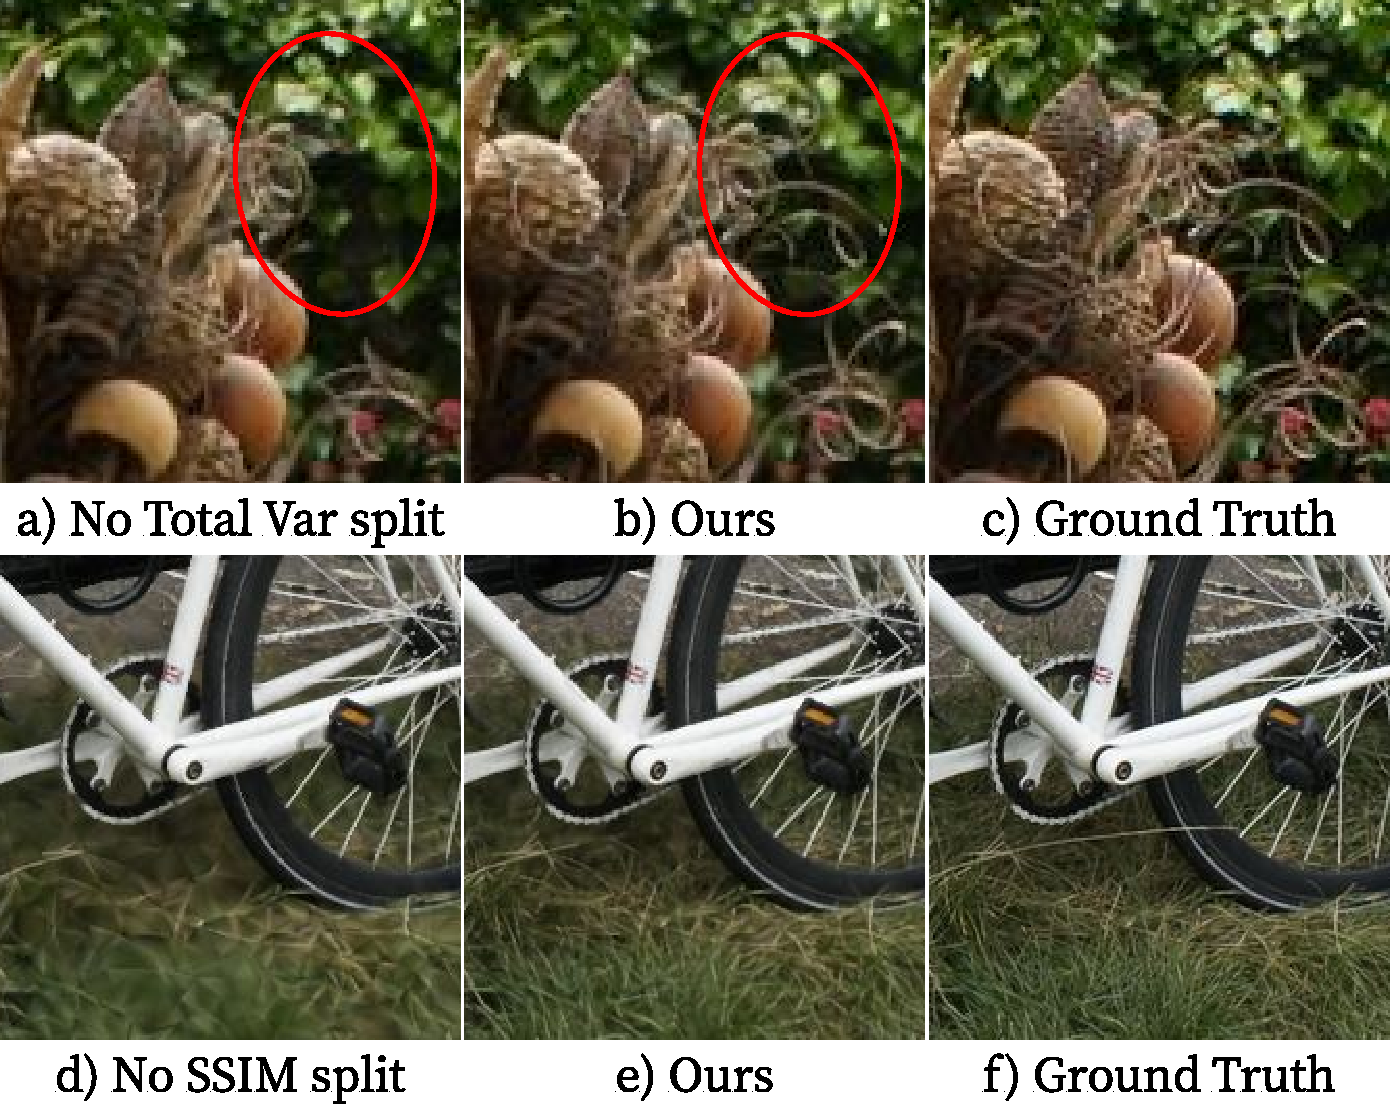
\includegraphics[width=\linewidth]{figures/ablations.pdf}
    \vspace{-1em}
    \caption{Qualitative results of our ablation over our splitting methods. SSIM splitting handles texture, while total variance splitting handles thin structures. Red circles highlight missing detail}
    \label{fig:splitting_ablation}
\end{figure}

In Table~\ref{tab:ablations} we present our ablation study, run on the \textit{bicycle} and \textit{room} scenes, from Mip-NeRF360. We investigate different approaches for splitting and colorizing primitives, and different Instant-NGP querying approaches.
We see that omitting the SSIM based variance based densification (``SSIM Splitting") decreases performance significantly. Omitting the total dataset variance based densification (``Total Var Splitting") decreases performance marginally, and qualitatively mostly affects thin structures, shown in Fig.~\ref{fig:splitting_ablation}.
Assigning each tetrahedron a single color (``Constant Color'') instead of using a linear color results in a marginal decrease in quality.
Ablating the Instant-NGP (``No Instant-NGP'') and directly assigning properties to the vertices works poorly due to topology flips, as expected.
Ablating the downweighting used after in interpolation (``No Downweighting") hurts slightly.
(``No Centroid") is a test where we used the circumcenter instead of the centroid when querying the iNGP to get the value of each tet. As described in Sec.~\ref{sec:model}, the circumcenter is mathematically smooth but has worse numerical conditioning, a tradeoff that this experiment shows to be disadvantageous.

\begin{figure}[h]
    \centering
    \includegraphics[width=\linewidth]{figures/fps_ablation.pdf}
    \caption{We plot the frames per second across a wide range of resolutions that are common in modern hardware. We show how rendering tetrahedra with a tile-based approach similar to 3DGS is significantly slower than hardware-based rasterizers. We also show how  mesh shaders improve performance compared to instance-based rendering by reducing the number of duplicate memory loads.
    }
    \label{fig:speed_ablation}
\end{figure}

In Figure~\ref{fig:speed_ablation} we analyze different shader implementations to measure the impact of each choice. 
``Tile-based'' is a naive tile-based renderer that we adapted from the 3DGS SlangTorch codebase, and ``Instanced'' is a hardware triangle rasterizer with duplicated loads.
We see that switching from the tile-based renderer to the instanced hardware triangle rasterizer that utilizes vertex and fragment shaders yields a significant performance boost.
As detailed in Sec.~\ref{sec:model}, the standard rasterization pipeline incurs redundant primitive loads in the vertex shader.
We see that using our mesh shader pipeline eliminates this redundancy and achieves another significant performance gain.

\subsection{Capabilities}

Our model enables a variety of qualitative capabilities, all of which are shown in Figure~\ref{fig:capabilities}.

\myparagraph{Lens Models \& Ray Tracing}
Because our representation is highly general, we were able to straightforwardly implement a ray-tracer based on OptiX, by leveraging the transparency method from 3DGRT~\cite{3dgrt2024}. Crucially, our tetrahedral mesh allows us to utilize built-in hardware triangle intersection. We achieve 84 FPS on the MipNeRF 360 outdoor scenes and 190 FPS on the indoor scenes, at test resolution (roughly 720p on outdoor scenes, less than 1080p on indoor scenes). At comparable primitive counts, we achieve a 17\% speed increase relative to Radiant Foam's ray tracer. This enables us to train on arbitrary lenses.

\myparagraph{Surface mesh extraction}
Our volumetric representation can be converted into a surface mesh using a straightforward procedure: We measure the peak color contribution of each tetrahedron across all pixels and all training views. We use this quantity to then threshold the radiance mesh by removing the tetrahedrons with a smaller peak color contribution than $0.1$. We then identify the connected components of all tetrahedra and construct a surface mesh for each one.

\myparagraph{Deformation and Simulation}
Finite element analysis and various simulation techniques like Position Based Dynamics (PBD)~\cite{muller2007position, macklin2016xpbd} are proven to be very useful and practical in interactive graphics applications. We demonstrate in Fig.~\ref{fig:capabilities} that a radiance mesh can directly use PBD and xPDB techniques to create interactive physical simulators, we also provide recorded interactive sessions in our supplemental video. This is a direct consequence of the nature of radiance meshes, as we are using the primal form of the Voronoi diagram --- a simple Tetrahedral mesh. Previous work~\cite{govindarajan2025radiant} that use the dual form of a Voronoi diagram only store, optimize, and render the generators of each cell. Animating these generator sites would cause non-trivial topological changes to the cell shapes. 

%However, the representation used by Radiant Foam~\cite{govindarajan2025radiant} is in its dual form, which lacks explicit vertices \jb{this reads like a complete non-sequitor, why are you bringing up Radiant Foam?}; it only stores, optimizes, and renders the generators of each cell. Animating these generator sites causes non-trivial topological changes to the cell shapes. Furthermore, switching from the dual to the primal form for simulation would break the Radiant Foam rendering method and introduce tens of millions of polyhedral faces, which are expensive to render as they require triangulation.

%In contrast, our method optimizes and renders the primal form directly. This allows us to apply methods like PBD and xPBD natively to our \longnamesingular{} and view the results using our standard rendering techniques, as shown on the right of Fig.~\ref{fig:capabilities}.

%\jb{You should rewrite this whole section so that you first spend many words explaining how your model works well for this, and then you should briefly explain why prior work doesn't do this, instead of the opposite.}

\begin{figure}
    \centering
    \includegraphics[width=\linewidth]{figures/capabilities.pdf}
    \caption{Radiance meshes enable a variety of useful capabilities. 
    Bottom left: our splatting method supports fisheye during training because power sorting supports any camera where rays share a common origin.
    Bottom right: Blender rendering of a surface mesh of the \scenename{bicycle} scene obtained by thresholding the scene.
    Top right: To simulate physics in realtime, we apply xPBD~\cite{macklin2016xpbd} to the radiance mesh vertices.}
    \label{fig:capabilities}
\end{figure}


% \begin{figure*}
%     \centering
%     \includegraphics[width=\linewidth]{figures/FPS.pdf}
%     \caption{Mesh rendering is not available on the NVIDIA A5000. As a result, we fallback to instanced rendering. A5000 results are not up to date yet.}
%     \label{fig:fps}
% \end{figure*}


\section{Conclusion}

We have presented radiance meshes, a novel hybrid radiance field representation that leverages the Delaunay triangulation to surpass the speed and flexibility of fast particle-based approaches, while still providing the physical consistency, and the lack of temporal artifacts of much slower neural field approaches. To accomplish this, we have presented a novel way to parameterize the attributes of the tetrahedra yielded by a Delaunay triangulation using an Instant-NGP. We additionally presented techniques for tetrahedral densification and hardware accelerated tetrahedral rendering.
We have shown that this flexible backwards-compatible representation enables a variety of standard editing applications and physics-based simulation approaches, in addition to supporting arbitrary lens distortions.
We believe that our approach represents a compelling combination of highly desirable properties for radiance field models, and we hope that this work will bring the community closer to widespread adoption of radiance field techniques in user-facing computer graphics applications.

\iftoggle{iccvfinal}{
\myparagraph{Acknowledgements}
We would like to thank the GraphDeco team at Inria, for providing a stimulating research environment during the final three months of this work.
AM is funded in part by the USACE Engineer Research and Development Center Cooperative Agreement W9132T-22-2-0014. AM conducted the final steps of research at GraphDeco@Inria.
}{}


% \section{Limitations and Future Work}

% {\bf Training Efficiency}: Our training pipeline has significant room for optimization. The billboard-based differentiable renderer used during training is a performance bottleneck, and fully recomputing the Delaunay triangulation at each iteration—without leveraging temporal coherence from previous steps — causes significant computational overhead.

% {\bf Backbone Dependency}: Reliance on the Instant-NGP backbone caps both maximum reconstruction quality and training speed, as querying the hash grid for per-cell attributes introduces latency.

% {\bf Deformation and Sorting}: While our approach supports editing and mesh deformation, significant perturbations can alter tetrahedron circumspheres, potentially invalidating the visibility sorting order required for correct rasterization. As a result, various downstream operations must be carefully designed to overcome this limitation.

% Extracting a manifold surface mesh out of the tetrahedron set would enable mathrmure and geometry optimization of the final representation, but represents a challenging task. 
% \section{Limitations}
% Perturbations to the \longnamesingular{} can change the circumsphere centers, which can change the sort order of the tetrahedra. As a result, various downstream operations must be carefully designed to overcome this limitation.

% The instant-NGP backbone limits the quality significantly. The quality is very sensitive to changes to parameters in this backbone, and it seems to be holding the method back. The optimization technique does not seem to be ideal.

% \section{Conclusion}
% Our approach to volume rendering using a Delaunay triangulation is able to hit incredibly high rasterization speeds, able to rasterize a \longnamesingular{} with twice as many primitives at the same speed.

% Compared to Radiant Foam, the other mesh based view synthesis method that uses a Voronoi diagram, our 
% Our method is dual to the approach
% Max primitives reliably supported with a GPU with 24GB of VRAM is 3.3 million. Our approach supports 13 million.
% Even with nearly 4 times as many primitives, our method matches the rendering speed at the test set resolution, while gaining an advantage as resolution increases. Our approach is 2x faster at 4k.

% \section{Future Work}
% Training speed has tons of low hanging fruit, as the billboard based differentiable rendering is highly suboptimal, and restarting the Delaunay triangulation without knowledge of the previous iteration is not ideal.
% Once the tetrahedra mesh has been optimized, there is much more flexibility in how the model can be represented. A lot of performance can be extracted by avoiding the need to duplicate the vertices and attach information about the entire tetrahedron to each of them.
% Extracting a manifold surface mesh out of the tetrahedron set would enable mathrmure and geometry optimization of the final representation, but represents a challenging task. 



{
    \small
    \bibliographystyle{ieeenat_fullname}
    \bibliography{main}
}

 


% WARNING: do not forget to delete the supplementary pages from your submission 
\clearpage
\setcounter{page}{1}
\maketitlesupplementary


\section{Backpropagation}
We use an adjoint rendering approach, starting from the last state of each ray, which we store, and reconstruct each ray state backwards using $p^{-1}(x, i)$. We can then use this reconstructed state to backpropagate the error to each state, then propagate this error to each primitive. The gradient with respect to mean, scale, and orientation, all come from the derivative of the ray-ellipsoid intersection function.  
To retrieve the list of primitives intersected, we store the list of intersections on the forward pass. Since rays tend to terminate before 300 total intersections, this turns out to be relatively cheap, at 1.2 KB per a ray. Although we experimented with using ray tracing to retrieve the list of surfaces in reverse order, we found the instability too high. 


\begin{figure*}[ht]
\centering
\bgroup
% \def\arraystretch{2}
\begin{tabular}{@{}c@{}c@{}c@{}c@{}c@{}}
\graphimtwelve{images/comparison_table_jpg/3DGS_im12.jpg} &
% \graphimtwelve{images/comparison_table_jpg/mcmc_im12.jpg} &
\graphimtwelve{images/comparison_table_jpg/stop_im12.jpg} &
% \graphimtwelve{images/comparison_table_jpg/3dgrt_im12.jpg} &
\graphimtwelve{images/comparison_table_jpg/smerf_im12.jpg} &
\graphimtwelve{images/comparison_table_jpg/ours_im12.jpg} &
\graphimtwelve{images/comparison_table_jpg/gt_im12.jpg} \\
% \raisebox{3.0cm}{\textbf{(b)}} &
\graphimthirteen{images/comparison_table_jpg/3DGS_im13.jpg} &
% \graphimthirteen{images/comparison_table_jpg/mcmc_im13.jpg} &
\graphimthirteen{images/comparison_table_jpg/stop_im13.jpg} &
% \graphimthirteen{images/comparison_table_jpg/3dgrt_im13.jpg} &
\graphimthirteen{images/comparison_table_jpg/smerf_im13.jpg} &
\graphimthirteen{images/comparison_table_jpg/ours_im13.jpg} &
\graphimthirteen{images/comparison_table_jpg/gt_im13.jpg} \\
% \graphimone{images/comparison_table_jpg/3DGS_im1.jpg} &
% \graphimone{images/comparison_table_jpg/mcmc_im1.jpg} &
% \graphimone{images/comparison_table_jpg/stop_im1.jpg} &
% \graphimone{images/comparison_table_jpg/ours_im1.jpg} &
% \graphimone{images/comparison_table_jpg/gt_im1.jpg} \\
\graphimseven{images/comparison_table_jpg/3DGS_im7.jpg} &
% \graphimseven{images/comparison_table_jpg/mcmc_im7.jpg} &
\graphimseven{images/comparison_table_jpg/stop_im7.jpg} &
% \graphimseven{images/comparison_table_jpg/3dgrt_im7.jpg} &
\graphimseven{images/comparison_table_jpg/smerf_im7.jpg} &
\graphimseven{images/comparison_table_jpg/ours_im7.jpg} &
\graphimseven{images/comparison_table_jpg/gt_im7.jpg} \\

\graphimfourteen{images/comparison_table_jpg/3DGS_im14.jpg} &
% \graphimfourteen{images/comparison_table_jpg/mcmc_im14.jpg} &
\graphimfourteen{images/comparison_table_jpg/stop_im14.jpg} &
% \graphimfourteen{images/comparison_table_jpg/3dgrt_im14.jpg} &
\graphimfourteen{images/comparison_table_jpg/smerf_im14.jpg} &
\graphimfourteen{images/comparison_table_jpg/ours_im14.jpg} &
\graphimfourteen{images/comparison_table_jpg/gt_im14.jpg} \\
% \graphimeleven{images/comparison_table_jpg/3DGS_im11.jpg} &
% \graphimeleven{images/comparison_table_jpg/mcmc_im11.jpg} &
% \graphimeleven{images/comparison_table_jpg/stop_im11.jpg} &
% \graphimeleven{images/comparison_table_jpg/ours_im11.jpg} &
% \graphimeleven{images/comparison_table_jpg/gt_im11.jpg} \\

% \graphimtwo{images/comparison_table_jpg/3DGS_im2.jpg} &
% \graphimtwo{images/comparison_table_jpg/mcmc_im2.jpg} &
% \graphimtwo{images/comparison_table_jpg/stop_im2.jpg} &
% \graphimtwo{images/comparison_table_jpg/ours_im2.jpg} &
% \graphimtwo{images/comparison_table_jpg/gt_im2.jpg} \\

% \graphimnine{images/comparison_table_jpg/3DGS_im9.jpg} &
% % \graphimnine{images/comparison_table_jpg/mcmc_im9.jpg} &
% \graphimnine{images/comparison_table_jpg/stop_im9.jpg} &
% \graphimnine{images/comparison_table_jpg/ours_im9.jpg} &
% \graphimnine{images/comparison_table_jpg/gt_im9.jpg} \\
3DGS & StopThePop & SMERF & Ours & GT
\end{tabular}
\egroup
\caption{Additional visual comparison of our method on the Mip-NeRF 360 dataset~\cite{barron2023zip}.}
\label{fig:comparison_supp}
\end{figure*}

\begin{table*}[ht]
    \centering
    \begin{tabular}{l|rrrrr}
\rowcolor[HTML]{F1F3F4} 
\textbf{PSNR $\uparrow$}    & \multicolumn{1}{l}{\cellcolor[HTML]{F1F3F4}berlin} & \multicolumn{1}{l}{\cellcolor[HTML]{F1F3F4}nyc} & \multicolumn{1}{l}{\cellcolor[HTML]{F1F3F4}alameda} & \multicolumn{1}{l}{\cellcolor[HTML]{F1F3F4}london} & \multicolumn{1}{l}{\cellcolor[HTML]{F1F3F4}Average} \\ \hline
3DGS                        & \cellcolor[HTML]{FFFFB4}26.83                      & 26.90                                           & \cellcolor[HTML]{FFFFB4}24.14                       & 25.48                                              & 25.84                                               \\
Mip Splatting               & \cellcolor[HTML]{FFB3B3}27.30                      & \cellcolor[HTML]{FFD9B3}27.52                   & \cellcolor[HTML]{FFB3B3}24.76                       & \cellcolor[HTML]{FFD9B3}26.28                      & \cellcolor[HTML]{FFD9B3}26.46                       \\
StopThePop                  & 26.81                                              & \cellcolor[HTML]{FFFFB4}27.14                   & 24.12                                               & \cellcolor[HTML]{FFFFB4}25.61                      & \cellcolor[HTML]{FFFFB4}25.92                       \\
SMERF                       & 28.52                                              & \cellcolor[HTML]{FFFFB4}28.21                   & 25.35                                               & \cellcolor[HTML]{FFFFB4}27.05                      & \cellcolor[HTML]{FFFFB4}27.28                       \\
Ours                        & 27.24                                              & 27.93                                           & 24.72                                               & 26.49                                              & \cellcolor[HTML]{FFB3B3}26.60                       \\ \hline
Zip-NeRF                    & 28.59                                              & 28.42                                           & 25.41                                               & 27.06                                              & 27.37                                               \\ \hline
\rowcolor[HTML]{F1F3F4} 
\textbf{SSIM $\uparrow$}    & \multicolumn{1}{l}{\cellcolor[HTML]{F1F3F4}berlin} & \multicolumn{1}{l}{\cellcolor[HTML]{F1F3F4}nyc} & \multicolumn{1}{l}{\cellcolor[HTML]{F1F3F4}alameda} & \multicolumn{1}{l}{\cellcolor[HTML]{F1F3F4}london} & \multicolumn{1}{l}{\cellcolor[HTML]{F1F3F4}Average} \\ \hline
3DGS                        & .899                                               & .861                                            & .776                                                & .830                                               & .842                                                \\
Mip Splatting               & \cellcolor[HTML]{FFD9B3}.892                       & \cellcolor[HTML]{FFD9B3}.853                    & \cellcolor[HTML]{FFD9B3}.768                        & \cellcolor[HTML]{FFD9B3}.822                       & \cellcolor[HTML]{FFD9B3}.834                        \\
StopThePop                  & \cellcolor[HTML]{FFFFB4}.885                       & \cellcolor[HTML]{FFFFB4}.844                    & \cellcolor[HTML]{FFFFB4}.748                        & \cellcolor[HTML]{FFFFB4}.801                       & \cellcolor[HTML]{FFFFB4}.819                        \\
SMERF                       & \cellcolor[HTML]{FFFFB4}.887                       & \cellcolor[HTML]{FFFFB4}.844                    & \cellcolor[HTML]{FFFFB4}.758                        & \cellcolor[HTML]{FFFFB4}.829                       & \cellcolor[HTML]{FFFFB4}.830                        \\
Ours                        & \cellcolor[HTML]{FFB3B3}.900                       & \cellcolor[HTML]{FFB3B3}.863                    & \cellcolor[HTML]{FFB3B3}.779                        & \cellcolor[HTML]{FFB3B3}.837                       & \cellcolor[HTML]{FFB3B3}.845                        \\ \hline
Zip-NeRF                    & .891                                               & .850                                            & .767                                                & .835                                               & .836                                                \\ \hline
\rowcolor[HTML]{F1F3F4} 
\textbf{LPIPS $\downarrow$} & \multicolumn{1}{l}{\cellcolor[HTML]{F1F3F4}berlin} & \multicolumn{1}{l}{\cellcolor[HTML]{F1F3F4}nyc} & \multicolumn{1}{l}{\cellcolor[HTML]{F1F3F4}alameda} & \multicolumn{1}{l}{\cellcolor[HTML]{F1F3F4}london} & \multicolumn{1}{l}{\cellcolor[HTML]{F1F3F4}Average} \\ \hline
3DGS                        & \cellcolor[HTML]{FFFFB4}.406                       & \cellcolor[HTML]{FFFFB4}.380                    & \cellcolor[HTML]{FFFFB4}.441                        & \cellcolor[HTML]{FFFFB4}.446                       & \cellcolor[HTML]{FFFFB4}.418                        \\
Mip Splatting               & .392                                               & .356                                            & .410                                                & .411                                               & .392                                                \\
StopThePop                  & \cellcolor[HTML]{FFD9B3}.402                       & \cellcolor[HTML]{FFD9B3}.373                    & \cellcolor[HTML]{FFD9B3}.433                        & \cellcolor[HTML]{FFD9B3}.438                       & \cellcolor[HTML]{FFD9B3}.411                        \\
SMERF                       & \cellcolor[HTML]{FFD9B3}.391                       & \cellcolor[HTML]{FFD9B3}.361                    & \cellcolor[HTML]{FFD9B3}.416                        & \cellcolor[HTML]{FFD9B3}.390                       & \cellcolor[HTML]{FFD9B3}.389                        \\
Ours                        & \cellcolor[HTML]{FFB3B3}.371                       & \cellcolor[HTML]{FFB3B3}.337                    & \cellcolor[HTML]{FFB3B3}.389                        & \cellcolor[HTML]{FFB3B3}.374                       & \cellcolor[HTML]{FFB3B3}.368                        \\ \hline
Zip-NeRF                    & .378                                               & .331                                            & .387                                                & .360                                               & .364                                               
\end{tabular}
    \caption{Full results for Zip-NeRF dataset}
    % \label{tab:full_zipnerf}
    \centering
    \begin{tabular}{l|rrrrr|rrrr}
\rowcolor[HTML]{F1F3F4} 
\textbf{PSNR $\uparrow$}    & \multicolumn{1}{l}{\cellcolor[HTML]{F1F3F4}bicycle} & \multicolumn{1}{l}{\cellcolor[HTML]{F1F3F4}flowers} & \multicolumn{1}{l}{\cellcolor[HTML]{F1F3F4}garden} & \multicolumn{1}{l}{\cellcolor[HTML]{F1F3F4}stump} & \multicolumn{1}{l|}{\cellcolor[HTML]{F1F3F4}treehill} & \multicolumn{1}{l}{\cellcolor[HTML]{F1F3F4}room} & \multicolumn{1}{l}{\cellcolor[HTML]{F1F3F4}counter} & \multicolumn{1}{l}{\cellcolor[HTML]{F1F3F4}kitchen} & \multicolumn{1}{l}{\cellcolor[HTML]{F1F3F4}bonsai} \\ \hline
3DGS                        & \cellcolor[HTML]{FFFFB4}25.24                       & 21.55                                               & \cellcolor[HTML]{FFFFB4}27.38                      & 26.56                                             & 22.43                                                 & \cellcolor[HTML]{FFD9B3}31.53                    & \cellcolor[HTML]{FFFFB4}29.00                       & \cellcolor[HTML]{FFD9B3}31.45                       & \cellcolor[HTML]{FFFFB4}32.21                      \\
StopThePop                  & 25.23                                               & \cellcolor[HTML]{FFFFB4}21.62                       & 27.33                                              & \cellcolor[HTML]{FFD9B3}26.65                     & \cellcolor[HTML]{FFFFB4}22.44                         & 30.91                                            & 28.79                                               & \cellcolor[HTML]{FFFFB4}31.13                       & 31.85                                              \\
3DGRT                       & 25.13                                               & 21.58                                               & 26.99                                              & \cellcolor[HTML]{FFFFB4}26.57                     & 22.40                                                 & 30.92                                            & 28.78                                               & 30.60                                               & 31.85                                              \\
SMERF                       & \cellcolor[HTML]{FFB3B3}25.58                       & \cellcolor[HTML]{FFB3B3}22.24                       & \cellcolor[HTML]{FFB3B3}27.66                      & \cellcolor[HTML]{FFB3B3}27.19                     & \cellcolor[HTML]{FFB3B3}23.93                         & \cellcolor[HTML]{FFFFB4}31.38                    & \cellcolor[HTML]{FFB3B3}29.02                       & \cellcolor[HTML]{FFB3B3}31.68                       & \cellcolor[HTML]{FFB3B3}33.19                      \\
Our model                   & \cellcolor[HTML]{FFD9B3}25.34                       & \cellcolor[HTML]{FFD9B3}21.70                       & \cellcolor[HTML]{FFD9B3}27.46                      & 26.41                                             & \cellcolor[HTML]{FFD9B3}22.74                         & \cellcolor[HTML]{FFB3B3}31.39                    & \cellcolor[HTML]{FFD9B3}28.91                       & 31.36                                               & \cellcolor[HTML]{FFD9B3}32.24                      \\ \hline
ZipNeRF                     & 25.80                                               & 22.40                                               & 28.20                                              & 27.55                                             & 23.89                                                 & 32.65                                            & 29.38                                               & 32.50                                               & 34.46                                              \\ \hline
\rowcolor[HTML]{F1F3F4} 
\textbf{SSIM $\uparrow$}    & \multicolumn{1}{l}{\cellcolor[HTML]{F1F3F4}bicycle} & \multicolumn{1}{l}{\cellcolor[HTML]{F1F3F4}flowers} & \multicolumn{1}{l}{\cellcolor[HTML]{F1F3F4}garden} & \multicolumn{1}{l}{\cellcolor[HTML]{F1F3F4}stump} & \multicolumn{1}{l|}{\cellcolor[HTML]{F1F3F4}treehill} & \multicolumn{1}{l}{\cellcolor[HTML]{F1F3F4}room} & \multicolumn{1}{l}{\cellcolor[HTML]{F1F3F4}counter} & \multicolumn{1}{l}{\cellcolor[HTML]{F1F3F4}kitchen} & \multicolumn{1}{l}{\cellcolor[HTML]{F1F3F4}bonsai} \\ \hline
3DGS                        & .766                                                & .606                                                & \cellcolor[HTML]{FFD9B3}.866                       & .771                                              & .633                                                  & \cellcolor[HTML]{FFD9B3}.919                     & \cellcolor[HTML]{FFD9B3}.909                        & \cellcolor[HTML]{FFB3B3}.928                        & \cellcolor[HTML]{FFB3B3}.942                       \\
StopThePop                  & \cellcolor[HTML]{FFFFB4}.768                        & .607                                                & \cellcolor[HTML]{FFD9B3}.866                       & .775                                              & .635                                                  & \cellcolor[HTML]{FFD9B3}.919                     & .907                                                & \cellcolor[HTML]{FFD9B3}.927                        & \cellcolor[HTML]{FFFFB4}.941                       \\
3DGRT                       & \cellcolor[HTML]{FFD9B3}.770                        & \cellcolor[HTML]{FFFFB4}.624                        & \cellcolor[HTML]{FFFFB4}.858                       & \cellcolor[HTML]{FFFFB4}.779                      & \cellcolor[HTML]{FFFFB4}.636                          & .917                                             & \cellcolor[HTML]{FFFFB4}.908                        & .924                                                & \cellcolor[HTML]{FFB3B3}.942                       \\
SMERF                       & .760                                                & \cellcolor[HTML]{FFD9B3}.626                        & .844                                               & \cellcolor[HTML]{FFB3B3}.784                      & \cellcolor[HTML]{FFB3B3}.682                          & \cellcolor[HTML]{FFFFB4}.918                     & .892                                                & .916                                                & \cellcolor[HTML]{FFFFB4}.941                       \\
Our model                   & \cellcolor[HTML]{FFB3B3}.776                        & \cellcolor[HTML]{FFB3B3}.639                        & \cellcolor[HTML]{FFB3B3}.869                       & \cellcolor[HTML]{FFD9B3}.781                      & \cellcolor[HTML]{FFD9B3}.656                          & \cellcolor[HTML]{FFB3B3}.922                     & \cellcolor[HTML]{FFB3B3}.910                        & \cellcolor[HTML]{FFFFB4}.926                        & \cellcolor[HTML]{FFD9B3}.943                       \\ \hline
ZipNeRF                     & .769                                                & .642                                                & .860                                               & .800                                              & .681                                                  & .925                                             & .902                                                & .928                                                & .949                                               \\ \hline
\rowcolor[HTML]{F1F3F4} 
\textbf{LPIPS $\downarrow$} & \multicolumn{1}{l}{\cellcolor[HTML]{F1F3F4}bicycle} & \multicolumn{1}{l}{\cellcolor[HTML]{F1F3F4}flowers} & \multicolumn{1}{l}{\cellcolor[HTML]{F1F3F4}garden} & \multicolumn{1}{l}{\cellcolor[HTML]{F1F3F4}stump} & \multicolumn{1}{l|}{\cellcolor[HTML]{F1F3F4}treehill} & \multicolumn{1}{l}{\cellcolor[HTML]{F1F3F4}room} & \multicolumn{1}{l}{\cellcolor[HTML]{F1F3F4}counter} & \multicolumn{1}{l}{\cellcolor[HTML]{F1F3F4}kitchen} & \multicolumn{1}{l}{\cellcolor[HTML]{F1F3F4}bonsai} \\ \hline
3DGS                        & .240                                                & .367                                                & \cellcolor[HTML]{FFD9B3}.123                       & .251                                              & .376                                                  & .287                                             & .258                                                & \cellcolor[HTML]{FFD9B3}.155                        & .252                                               \\
StopThePop                  & \cellcolor[HTML]{FFFFB4}.233                        & .362                                                & \cellcolor[HTML]{FFB3B3}.120                       & \cellcolor[HTML]{FFFFB4}.244                      & .366                                                  & .281                                             & \cellcolor[HTML]{FFFFB4}.253                        & \cellcolor[HTML]{FFB3B3}.154                        & .249                                               \\
3DGRT                       & \cellcolor[HTML]{FFD9B3}.226                        & \cellcolor[HTML]{FFFFB4}.335                        & \cellcolor[HTML]{FFFFB4}.134                       & \cellcolor[HTML]{FFD9B3}.243                      & \cellcolor[HTML]{FFFFB4}.364                          & \cellcolor[HTML]{FFFFB4}.280                     & \cellcolor[HTML]{FFD9B3}.248                        & \cellcolor[HTML]{FFFFB4}.156                        & \cellcolor[HTML]{FFFFB4}.242                       \\
SMERF                       & .239                                                & \cellcolor[HTML]{FFD9B3}.317                        & .147                                               & \cellcolor[HTML]{FFD9B3}.243                      & \cellcolor[HTML]{FFB3B3}.302                          & \cellcolor[HTML]{FFB3B3}.259                     & .256                                                & \cellcolor[HTML]{FFD9B3}.155                        & \cellcolor[HTML]{FFB3B3}.222                       \\
Our model                   & \cellcolor[HTML]{FFB3B3}.220                        & \cellcolor[HTML]{FFB3B3}.307                        & \cellcolor[HTML]{FFB3B3}.120                       & \cellcolor[HTML]{FFB3B3}.230                      & \cellcolor[HTML]{FFD9B3}.318                          & \cellcolor[HTML]{FFD9B3}.275                     & \cellcolor[HTML]{FFB3B3}.240                        & \cellcolor[HTML]{FFD9B3}.155                        & \cellcolor[HTML]{FFD9B3}.236                       \\ \hline
ZipNeRF                     & .228                                                & .309                                                & .127                                               & .236                                              & .281                                                  & .238                                             & .223                                                & .134                                                & .196                                              
\end{tabular}
    \caption{Full results for Mip-NeRF 360 dataset}
    \label{tab:full_mipnerf}
\end{table*}

\section{Hyperparameters, Etc} \label{sec:hparams}
We change the opacity learning rate to $0.0125$, the initial position learning rate to $4\times10^{-5}$ and the final position learning rate to $4\times10^{-7}$. We change the parameter known as ``percent dense'' in 3DGS to $0.001785$, which controls the size threshold above which primitives are split instead of cloned. We perform this every 200 iterations, instead of 100, and set the splitting gradient threshold to $2.5\times10^{-7}$ and the clone gradient threshold to $0.1$. We also stop splitting and cloning at 7 million primitives, or at 16000 iterations, which ever comes first, and start at 1500 iterations.

For color, we apply a softplus activation ($\beta=10$) to the output of the spherical harmonics (instead of 3DGS's relu activation), which we find avoids certain local minima where primitives get locked into a color. We increase the spherical harmonic degree every $2,\!000$ iterations, instead of $1,\!000$. We set the max primitive size to $25$ units, which improves performance.


\subsection{Inverse Contraction Initialization}
To help initialize the primitives in a scene, we supplement the SfM initialization with $10,\!000$ additional primitives. We generate these primitives by sampling their means uniformly from a radius-2 sphere. The radius is set to a constant value based the max radius at which the spheres could be packed into the radius-2 sphere, and colors are set to a constant value of $0.5$.
These primitives are then transformed by ``uncontracting'' the resulting means and covariances using the inverse of the contraction used in mip-NeRF 360~\cite{barron2022mip}. We found that highly anisotropic primitives at initialization can cause issues, so we scale the primitives to be isotropic.

To review, the mip-NeRF 360 contraction function $\mathcal{C}$ that maps from a 3D coordinate in Euclidean space $\mathbf{x}$ to a 3D coordinate in contracted space $\mathbf{z}$ is:
\begin{equation}
  \mathcal{C}(\mathbf{x}) = \mathbf{x} \cdot \frac{2 \sqrt{\max(1, || \mathbf{x} ||^2)} - 1}{\max(1, || \mathbf{x} ||^2)}
\end{equation}
The inverse of $\mathcal{C}(\mathbf{x})$ can be defined straightforwardly:
\begin{equation}
    \mathcal{C}^{-1}(\mathbf{z}) = \frac{\mathbf{z}}{\sqrt{\max(1, ||\mathbf{z}||^2)} (2 - \min(2, \sqrt{\max(1, ||\mathbf{z}||^2)}))}
\end{equation}
To apply this inverse contraction to a Gaussian instead of a point, we use the same Kalman-esque approach as was used in mip-NeRF 360: we linearize the contraction around $\mathbf{z}$ into a Jacobian-vector product, which we apply twice to the input covariance matrix.


\end{document}
